% TEMPLATE for Usenix papers, specifically to meet requirements of
%  USENIX '05
% originally a template for producing IEEE-format articles using LaTeX.
%   written by Matthew Ward, CS Department, Worcester Polytechnic Institute.
% adapted by David Beazley for his excellent SWIG paper in Proceedings,
%   Tcl 96
% turned into a smartass generic template by De Clarke, with thanks to
%   both the above pioneers
% use at your own risk.  Complaints to /dev/null.
% make it two column with no page numbering, default is 10 point

% Munged by Fred Douglis <douglis@research.att.com> 10/97 to separate
% the .sty file from the LaTeX source template, so that people can
% more easily include the .sty file into an existing document.  Also
% changed to more closely follow the style guidelines as represented
% by the Word sample file. 

% Note that since 2010, USENIX does not require endnotes. If you want
% foot of page notes, don't include the endnotes package in the 
% usepackage command, below.

% This version uses the latex2e styles, not the very ancient 2.09 stuff.
\documentclass[letterpaper,twocolumn,10pt]{article}
\usepackage{usenix,epsfig,endnotes}
\usepackage{graphicx,calc,subfigure,caption,float}
\usepackage[breaklinks,colorlinks]{hyperref}
\usepackage{endnotes,microtype,xspace,fancyvrb,multirow}
\usepackage{array,underscore,relsize}
\usepackage{booktabs,amsmath}
\usepackage{authblk}

\renewcommand{\ttdefault}{pxtt}

\newcommand{\URL}{\url}
\newcommand{\cc}[1]{\mbox{\smaller[0.5]\texttt{#1}}}

%\clubpenalty=10000
%\widowpenalty=10000

%\linespread{1.2}

\fvset{fontsize=\scriptsize,xleftmargin=8pt,numbers=left,numbersep=5pt}


\makeatletter
\def\PY@reset{\let\PY@it=\relax \let\PY@bf=\relax%
    \let\PY@ul=\relax \let\PY@tc=\relax%
    \let\PY@bc=\relax \let\PY@ff=\relax}
\def\PY@tok#1{\csname PY@tok@#1\endcsname}
\def\PY@toks#1+{\ifx\relax#1\empty\else%
    \PY@tok{#1}\expandafter\PY@toks\fi}
\def\PY@do#1{\PY@bc{\PY@tc{\PY@ul{%
    \PY@it{\PY@bf{\PY@ff{#1}}}}}}}
\def\PY#1#2{\PY@reset\PY@toks#1+\relax+\PY@do{#2}}

\expandafter\def\csname PY@tok@gd\endcsname{\def\PY@tc##1{\textcolor[rgb]{0.63,0.00,0.00}{##1}}}
\expandafter\def\csname PY@tok@gu\endcsname{\let\PY@bf=\textbf\def\PY@tc##1{\textcolor[rgb]{0.50,0.00,0.50}{##1}}}
\expandafter\def\csname PY@tok@gt\endcsname{\def\PY@tc##1{\textcolor[rgb]{0.00,0.27,0.87}{##1}}}
\expandafter\def\csname PY@tok@gs\endcsname{\let\PY@bf=\textbf}
\expandafter\def\csname PY@tok@gr\endcsname{\def\PY@tc##1{\textcolor[rgb]{1.00,0.00,0.00}{##1}}}
\expandafter\def\csname PY@tok@cm\endcsname{\let\PY@it=\textit\def\PY@tc##1{\textcolor[rgb]{0.25,0.50,0.50}{##1}}}
\expandafter\def\csname PY@tok@vg\endcsname{\def\PY@tc##1{\textcolor[rgb]{0.10,0.09,0.49}{##1}}}
\expandafter\def\csname PY@tok@m\endcsname{\def\PY@tc##1{\textcolor[rgb]{0.40,0.40,0.40}{##1}}}
\expandafter\def\csname PY@tok@mh\endcsname{\def\PY@tc##1{\textcolor[rgb]{0.40,0.40,0.40}{##1}}}
\expandafter\def\csname PY@tok@go\endcsname{\def\PY@tc##1{\textcolor[rgb]{0.53,0.53,0.53}{##1}}}
\expandafter\def\csname PY@tok@ge\endcsname{\let\PY@it=\textit}
\expandafter\def\csname PY@tok@vc\endcsname{\def\PY@tc##1{\textcolor[rgb]{0.10,0.09,0.49}{##1}}}
\expandafter\def\csname PY@tok@il\endcsname{\def\PY@tc##1{\textcolor[rgb]{0.40,0.40,0.40}{##1}}}
\expandafter\def\csname PY@tok@cs\endcsname{\let\PY@it=\textit\def\PY@tc##1{\textcolor[rgb]{0.25,0.50,0.50}{##1}}}
\expandafter\def\csname PY@tok@cp\endcsname{\def\PY@tc##1{\textcolor[rgb]{0.74,0.48,0.00}{##1}}}
\expandafter\def\csname PY@tok@gi\endcsname{\def\PY@tc##1{\textcolor[rgb]{0.00,0.63,0.00}{##1}}}
\expandafter\def\csname PY@tok@gh\endcsname{\let\PY@bf=\textbf\def\PY@tc##1{\textcolor[rgb]{0.00,0.00,0.50}{##1}}}
\expandafter\def\csname PY@tok@ni\endcsname{\let\PY@bf=\textbf\def\PY@tc##1{\textcolor[rgb]{0.60,0.60,0.60}{##1}}}
\expandafter\def\csname PY@tok@nl\endcsname{\def\PY@tc##1{\textcolor[rgb]{0.63,0.63,0.00}{##1}}}
\expandafter\def\csname PY@tok@nn\endcsname{\let\PY@bf=\textbf\def\PY@tc##1{\textcolor[rgb]{0.00,0.00,1.00}{##1}}}
\expandafter\def\csname PY@tok@no\endcsname{\def\PY@tc##1{\textcolor[rgb]{0.53,0.00,0.00}{##1}}}
\expandafter\def\csname PY@tok@na\endcsname{\def\PY@tc##1{\textcolor[rgb]{0.49,0.56,0.16}{##1}}}
\expandafter\def\csname PY@tok@nb\endcsname{\def\PY@tc##1{\textcolor[rgb]{0.00,0.50,0.00}{##1}}}
\expandafter\def\csname PY@tok@nc\endcsname{\let\PY@bf=\textbf\def\PY@tc##1{\textcolor[rgb]{0.00,0.00,1.00}{##1}}}
\expandafter\def\csname PY@tok@nd\endcsname{\def\PY@tc##1{\textcolor[rgb]{0.67,0.13,1.00}{##1}}}
\expandafter\def\csname PY@tok@ne\endcsname{\let\PY@bf=\textbf\def\PY@tc##1{\textcolor[rgb]{0.82,0.25,0.23}{##1}}}
\expandafter\def\csname PY@tok@nf\endcsname{\def\PY@tc##1{\textcolor[rgb]{0.00,0.00,1.00}{##1}}}
\expandafter\def\csname PY@tok@si\endcsname{\let\PY@bf=\textbf\def\PY@tc##1{\textcolor[rgb]{0.73,0.40,0.53}{##1}}}
\expandafter\def\csname PY@tok@s2\endcsname{\def\PY@tc##1{\textcolor[rgb]{0.73,0.13,0.13}{##1}}}
\expandafter\def\csname PY@tok@vi\endcsname{\def\PY@tc##1{\textcolor[rgb]{0.10,0.09,0.49}{##1}}}
\expandafter\def\csname PY@tok@nt\endcsname{\let\PY@bf=\textbf\def\PY@tc##1{\textcolor[rgb]{0.00,0.50,0.00}{##1}}}
\expandafter\def\csname PY@tok@nv\endcsname{\def\PY@tc##1{\textcolor[rgb]{0.10,0.09,0.49}{##1}}}
\expandafter\def\csname PY@tok@s1\endcsname{\def\PY@tc##1{\textcolor[rgb]{0.73,0.13,0.13}{##1}}}
\expandafter\def\csname PY@tok@sh\endcsname{\def\PY@tc##1{\textcolor[rgb]{0.73,0.13,0.13}{##1}}}
\expandafter\def\csname PY@tok@sc\endcsname{\def\PY@tc##1{\textcolor[rgb]{0.73,0.13,0.13}{##1}}}
\expandafter\def\csname PY@tok@sx\endcsname{\def\PY@tc##1{\textcolor[rgb]{0.00,0.50,0.00}{##1}}}
\expandafter\def\csname PY@tok@bp\endcsname{\def\PY@tc##1{\textcolor[rgb]{0.00,0.50,0.00}{##1}}}
\expandafter\def\csname PY@tok@c1\endcsname{\let\PY@it=\textit\def\PY@tc##1{\textcolor[rgb]{0.25,0.50,0.50}{##1}}}
\expandafter\def\csname PY@tok@kc\endcsname{\let\PY@bf=\textbf\def\PY@tc##1{\textcolor[rgb]{0.00,0.50,0.00}{##1}}}
\expandafter\def\csname PY@tok@c\endcsname{\let\PY@it=\textit\def\PY@tc##1{\textcolor[rgb]{0.25,0.50,0.50}{##1}}}
\expandafter\def\csname PY@tok@mf\endcsname{\def\PY@tc##1{\textcolor[rgb]{0.40,0.40,0.40}{##1}}}
\expandafter\def\csname PY@tok@err\endcsname{\def\PY@bc##1{\setlength{\fboxsep}{0pt}\fcolorbox[rgb]{1.00,0.00,0.00}{1,1,1}{\strut ##1}}}
\expandafter\def\csname PY@tok@kd\endcsname{\let\PY@bf=\textbf\def\PY@tc##1{\textcolor[rgb]{0.00,0.50,0.00}{##1}}}
\expandafter\def\csname PY@tok@ss\endcsname{\def\PY@tc##1{\textcolor[rgb]{0.10,0.09,0.49}{##1}}}
\expandafter\def\csname PY@tok@sr\endcsname{\def\PY@tc##1{\textcolor[rgb]{0.73,0.40,0.53}{##1}}}
\expandafter\def\csname PY@tok@mo\endcsname{\def\PY@tc##1{\textcolor[rgb]{0.40,0.40,0.40}{##1}}}
\expandafter\def\csname PY@tok@kn\endcsname{\let\PY@bf=\textbf\def\PY@tc##1{\textcolor[rgb]{0.00,0.50,0.00}{##1}}}
\expandafter\def\csname PY@tok@mi\endcsname{\def\PY@tc##1{\textcolor[rgb]{0.40,0.40,0.40}{##1}}}
\expandafter\def\csname PY@tok@gp\endcsname{\let\PY@bf=\textbf\def\PY@tc##1{\textcolor[rgb]{0.00,0.00,0.50}{##1}}}
\expandafter\def\csname PY@tok@o\endcsname{\def\PY@tc##1{\textcolor[rgb]{0.40,0.40,0.40}{##1}}}
\expandafter\def\csname PY@tok@kr\endcsname{\let\PY@bf=\textbf\def\PY@tc##1{\textcolor[rgb]{0.00,0.50,0.00}{##1}}}
\expandafter\def\csname PY@tok@s\endcsname{\def\PY@tc##1{\textcolor[rgb]{0.73,0.13,0.13}{##1}}}
\expandafter\def\csname PY@tok@kp\endcsname{\def\PY@tc##1{\textcolor[rgb]{0.00,0.50,0.00}{##1}}}
\expandafter\def\csname PY@tok@w\endcsname{\def\PY@tc##1{\textcolor[rgb]{0.73,0.73,0.73}{##1}}}
\expandafter\def\csname PY@tok@kt\endcsname{\def\PY@tc##1{\textcolor[rgb]{0.69,0.00,0.25}{##1}}}
\expandafter\def\csname PY@tok@ow\endcsname{\let\PY@bf=\textbf\def\PY@tc##1{\textcolor[rgb]{0.67,0.13,1.00}{##1}}}
\expandafter\def\csname PY@tok@sb\endcsname{\def\PY@tc##1{\textcolor[rgb]{0.73,0.13,0.13}{##1}}}
\expandafter\def\csname PY@tok@k\endcsname{\let\PY@bf=\textbf\def\PY@tc##1{\textcolor[rgb]{0.00,0.50,0.00}{##1}}}
\expandafter\def\csname PY@tok@se\endcsname{\let\PY@bf=\textbf\def\PY@tc##1{\textcolor[rgb]{0.73,0.40,0.13}{##1}}}
\expandafter\def\csname PY@tok@sd\endcsname{\let\PY@it=\textit\def\PY@tc##1{\textcolor[rgb]{0.73,0.13,0.13}{##1}}}

\def\PYZbs{\char`\\}
\def\PYZus{\char`\_}
\def\PYZob{\char`\{}
\def\PYZcb{\char`\}}
\def\PYZca{\char`\^}
\def\PYZam{\char`\&}
\def\PYZlt{\char`\<}
\def\PYZgt{\char`\>}
\def\PYZsh{\char`\#}
\def\PYZpc{\char`\%}
\def\PYZdl{\char`\$}
\def\PYZhy{\char`\-}
\def\PYZsq{\char`\'}
\def\PYZdq{\char`\"}
\def\PYZti{\char`\~}
% for compatibility with earlier versions
\def\PYZat{@}
\def\PYZlb{[}
\def\PYZrb{]}
\makeatother


\newcommand{\figrule}{\hrule width \hsize height .33pt}
\newcommand{\coderule}{\vspace{-0.4em}\figrule}

\setlength{\abovedisplayskip}{0pt}
\setlength{\abovedisplayshortskip}{0pt}
\setlength{\belowdisplayskip}{0pt}
\setlength{\belowdisplayshortskip}{0pt}
\setlength{\jot}{0pt}

\def\Snospace~{\S{}}
\renewcommand*\sectionautorefname{\Snospace}
\def\sectionautorefname{\Snospace}
\def\subsectionautorefname{\Snospace}
\def\subsubsectionautorefname{\Snospace}
\def\chapterautorefname{\Snospace}
%\renewcommand{\figurename}{Fig.}
%\def\figureautorefname{\figurename}
\newcommand{\subfigureautorefname}{\figureautorefname}

%\numberwithin{equation}{section}
\newcommand{\yes}{Y}
\newcommand{\no}{}

% sema
\newcommand{\shl}{\ \cc{<}\cc{<}\ }
\newcommand{\shr}{\ \cc{>}\cc{>}\ }

\if 0
\renewcommand{\topfraction}{0.9}
\renewcommand{\dbltopfraction}{0.9}
\renewcommand{\bottomfraction}{0.8}
\renewcommand{\textfraction}{0.05}
\renewcommand{\floatpagefraction}{0.9}
\renewcommand{\dblfloatpagefraction}{0.9}
\setcounter{topnumber}{10}
\setcounter{bottomnumber}{10}
\setcounter{totalnumber}{10}
\setcounter{dbltopnumber}{10}
\fi

\newif\ifdraft\drafttrue
\newif\ifnotes\notestrue
\ifdraft\else\notesfalse\fi

% ref. http://en.wikibooks.org/wiki/LaTeX/Colors
\newcommand{\TK}[1]{\textcolor{LimeGreen}{TK: #1}}
\newcommand{\BL}[1]{\textcolor{LimeGreen}{BL: #1}}
\newcommand{\CS}[1]{\textcolor{LimeGreen}{CS: #1}}
\newcommand{\YJ}[1]{\textcolor{LimeGreen}{YJ: #1}}
\newcommand{\KLU}[1]{\textcolor{LimeGreen}{KLU: #1}}
\newcommand{\XXX}[1]{\textcolor{red}{XXX: #1}}
\newcommand{\TODO}[1]{\textcolor{Melon}{TODO: #1}}

% hide comments
% \renewcommand{\TK}[1]{\ignorespaces}
% \renewcommand{\XXX}[1]{\ignorespaces}
% \renewcommand{\TODO}[1]{\ignorespaces}

%% Ensure ligatures (e.g., ``fine official flag'') can be copy/pasted from PDF.

% Ruian
%\input{glyphtounicode}
%\pdfgentounicode=1

\newcolumntype{R}[1]{>{\raggedleft\let\newline\\\arraybackslash\hspace{0pt}}p{#1}}

% include macros
\newcommand{\includepdf}[1]{
  \includegraphics[width=\columnwidth]{#1}
}
\newcommand{\includeplot}[1]{
  \resizebox{\columnwidth}{!}{\input{#1}}
}

% list
\newcommand{\squishlist}{
\begin{itemize}[noitemsep,nolistsep]
  \setlength{\itemsep}{-0pt}
}
\newcommand{\squishend}{
  \end{itemize}
}

\usepackage{float}
\floatstyle{plain}
\restylefloat{algorithm}

\newfloat{table}{thp}{lop}
\floatname{table}{\bf Table}
\def\tableautorefname{Table}

\newfloat{example}{thp}{lop}
\floatname{example}{\bf Example}
\def\exampleautorefname{Example}
\floatname{algorithm}{\bf Algorithm}

\newfloat{figure}{thp}{lop}
\floatname{figure}{\bf Figure}
\def\figureautorefname{Figure}

\newfloat{appendix}{}{lop}
\floatname{appendix}{\bf Appendix}
\def\appendixautorefname{Appendix}

\newcommand{\PP}[1]{
\noindent{\bf #1}
}

%%
%% NOTE.
%%  to use circled number in caption, use
%%   (e.g., \protect\C{1})
%%
\usepackage{tikz}
\newcommand*\C[1]{%
\begin{tikzpicture}[baseline=(C.base)]
\node[draw,circle,inner sep=0.3pt](C) {#1};
\end{tikzpicture}}


\begin{document}

%don't want date printed
\date{}

%make title bold and 14 pt font (Latex default is non-bold, 16 pt)
\title{\Large \bf SWM: Cloaking Detection through Simhash-based Website Model}
% Simhash-based Website Model: Towards Real-Time Cloaking Detection}
% Real-Time Cloaking Detection based on Simhash and Crowdsourcing

%for single author (just remove % characters)

%\author{
%{\rm Ruian Duan}\\
%\thanks{Georgia Institute of Technology}
%\and
%{\rm Weiren Wang}\\
%\thanks{Georgia Institute of Technology}
%\and
%{\rm Ji Zhang}\\
%\thanks{Google Inc.}
%\and
%{\rm Wenke Lee}\\
%\thanks{Georgia Institute of Technology}
%
%%wenke@cc.gatech.edu
%% copy the following lines to add more authors
%% \and
%% {\rm Name}\\
%%Name Institution
%} % end author
%



\author[*]{Ruian Duan}%\thanks{ruian@gatech.edu}}
\author[*]{Weiren Wang}%\thanks{weirenwang@gatech.edu}}
\author[**]{Ji Zhang}%\thanks{jiz@google.com}}
\author[*]{Wenke Lee}%\thanks{wenke@cc.gatech.edu}}
\affil[*]{Georgia Institute of Technology}
\affil[**]{Google Inc.}

\maketitle

% Use the following at camera-ready time to suppress page numbers.
% Comment it out when you first submit the paper for review.
\thispagestyle{empty}


\subsection*{Abstract}
Cloaking, used by spammers for the purpose of increasing exposure of
their websites, as well as to circumvent censorship, has been a notorious 
spamming search engine optimization technique. Recently, we also
identify a rising trend of employing cloaking in search engine marketing. The motivation of cloaking 
is to hide the true nature of a website by delivering blatantly different 
content to users versus censors. Cloaking is popular due to low setup cost 
and lack of efficient detection technique. 

In this paper, we propose Simhash-based Website Model, or SWM, a new way to
fuzzy hash the content and layout of a
website and model the dynamics of a website. 
We apply SWM in cloaking detection, and achieve 97.1\% true positive rate with
0.3\% false positive rate. 
SWM is more efficient compared to past approaches and can be deployed as browser
plugin for crowdsourcing user view of websites with negligible overhead.
In order to understand the incentives
behind cloaking, we systematically
categorize and review the detected samples, and find majority of them are
doing abusing search engine with traffic sale, and 4.3\% are 
malicious or phishing sites.
With motivation of both search engine and user to combat cloaking, we discuss
deployment of SWM in cloaking detection and
propose a novel model to
detect cloaking through crowdsourcing with user privacy guarantee.



\section{Introduction}
\label{s:intro}

Cloaking is a technique to deliver blatantly different content to users versus
censors on the web. 
Search engine is the main entry for user to get online today, and therefore,
attackers who want to promote illegal services or do phishing and malware
hosting is willing to have their page ranked high through search engine.
On the other hand, search engine develops algorithms to rank pages and penalize
these pages. In order to evade detection, attackers use cloaking to hide the
true nature of their website, conducting blackhat Search Engine Optimization (SEO).
Similarly, in Search Engine Marketing (SEM), advertisers pay search engine for
specific advertisements and get their page displayed on the first page of search
results. Attackers abuse this service to deliver non-compliant content to user.
The foundamental reason of SEO and SEM cloaking is that, search engine is just processing
information over the Internet, with no control over it, hence it is hard to
tell whether the copy of website that they see are actually what user sees.

In SEO and SEM, attackers use user agent, referer, IP etc based cloaking
techniques to avoid inspection. Among the cloaking techniques, IP cloaking is
very difficult to detect. 
There are two major challenges in cloaking detection in SEO and SEM.
First challenge is revealing the cloaked content. There are various
commercial tools, such as blackjack's, noIPfraud, and wpCloaker~\cite{intro:cloakware}
that are efficient in performing cloaking.
They provide different strategies of cloaking, including user agent, referer,
redirect, IP etc. Regarding IP cloaking, they provide services to periodically refresh the list of
crawlers' IP addresses. Therefore, revealing cloaked content is an ongoing war
between cloakers and censors.
Second challenge is differentiating
cloaking from naturally dynamic changes of the same page. Dynamic content is
allowed in SEO and SEM, however, blatantly deliver different, unrelated content
to search engine spider versus normal user is not allowed.

In order to address the first challenge, existing detection approaches pretend to be real user, e.g. set
referer, user agent, use multiple IPs or proxy to hide identity. But
attackers could identify them and incrementally blacklist IPs.
Intuitively, an alternate is to collect data from user side directly. However, it is hard
to collect sufficient data for comparison while protecting user privacy.
Regarding the second challenge, previous works go through the documents multiple times and compare page
difference to address the second challenge ~\cite{chellapilla2006improving, deng2013uncovering,
lin2009detection, wang2011cloak}.
There are mainly two shortcomings in previous approaches.
First,  they are slow, because pairwise comparison of documents is
computationally expensive and they usually require multiple passes of a
document.
Second, they are not suitable for crowdsourcing, because they may introduce
high overhead to user and violates user privacy. 

%To address the second challenge, ~\cite{wu2005cloaking} looks at the
%statistical features of a website, including words, tags, links. 
%~\cite{chellapilla2006improving} employs popular search words and high
%monetizable words to detect cloaking, say, detect cloaking in words that matter.
%~\cite{lin2009detection} looks at the tag sequence on a website.
%~\cite{wang2011cloak} employs text shingling, search snippet inclusion test in
%landing page and tag comparison to detect cloaking. However, these methods are
%either too naive, eg. look at statistics, or time-consuming and
%redundant~\cite{wang2011cloak}. Besides, since all these approaches are
%centralized detection, they can not be deployed to detect SEM cloaking, because
%the data collection phase, say, clicking search ads, actually results in click fraud.

This work employs simhash to address the two challenges.
Charikar's simhash ~\cite{charikar2002similarity} is a special signature of feature set. 
It is a class of Locality Sensitive Hash (LSH) that has been extensively used in
near duplicate in search engine.
It is an random projection based algorithm that maps high dimentional data to fixed bits while
maintaining the property that, hamming distance between the resulting bits is an
estimation of similarity between the original feature set.
%estimation of the Earth Mover Distance (EMD) between the original feature set.

%In our approach, we stand back and think about the dynamic nature of websites
%and try to figure out how can we measure or quantify the dynamics of websites.
%For example, does the change of a website follow some pattern? What is the
%average change? By answering these questions, we can then figure out the
%websites and then model them better. We first illustrate the dynamicness of a
%webpage and propose a way to model their change.
%Next, we train our model on manually label dataset to check some paramter to
%identify cloaking (one use case for website modeling). 
%Then, we employ our model to detect cloaking on advertisement cloaking dataset
%and identified \XXX{??} cloaking sites, showing prevalence of cloaking in both
%advertisements and search.
%
We propose Simhash-based Website Model(SWM) to model the dynamics of a
web page and use the outlier detection ability of SWM to do cloaking detection.
The basic idea is to generate two fuzzy hash corresponding to text and dom tree
for each website (fuzzy signature), and compare the differences between spider copy and user copy.
In order to model dynamics of a website, we retrieve spider copy multiple
times and leverage the fact that hamming distance is euclidean distance (
L1 norm) to learn patterns.
The proposed system achieves 97.1\% true positive rate with
0.3\% false positive rate.
%And much higher efficiency compared to past
%approaches. 

By applying the trained model on collected dataset, we detected 2600 cloaking samples in total.
Then, we manually classify and illustrate the incentives behind cloaking,
results show that the majority are doing blackhat SEO for traffic sale,
4.3\% of cloaking sites are malicious download or phishing sites. A breakdown of
the results are described in ~\autoref{s:measurement}.

With motivation of both search engine and user to combat cloaking, we propose a
novel model to collect simhash
%
%we establish incentives both search engine and users in cloaking detection.
%both user and search engine are interested in this.
%
from user side, with low overhead and privacy guarantee provided by RAPPOR.
By crowdsourcing the fuzzy signatures of what is actually shown to user, we
address both challenges in cloaking elegantly.

%In the new model, we can detect cloaking in SEM, because what we need to collect
%is url and statistics of simhash, which doesn't comply to click fraud. 

%Past approaches cannot handle advertisements, however, because of privacy issues
%and efficient hash technique. In comparison, our model is light-weight, easy to
%implement algorithm that can be used to fingerprint a website. And this
%fingerprint can be used to either compare against known blacklist, or send back
%to search engine for further analysis.
%


%According to ~\cite{lin2009detection}, many cloaking software packages support
%IP cloaking, and some even provide services to periodically refresh the list of
%crawlers’ IP addresses. Therefore, IP cloaking is hard to detect. To the
%author's knowledge, there is no known work that can solve IP
%cloaking.


%Security problems in cloaking, phishing site, suspicious site, non-compliant
%content, malware, dishonest behavior.
%
%Given a form to the user and tell him, you can get some money if you sigh up,
%but this form is not delivered to Google.

%Precision is 0.9610642439974043, out of 1541.
%
%This paper makes the following contributions:
%(1) Introduce simhash-based website model to represent the content and layout
%dynamics of a page.
%(2) Propose the idea and framework to detect cloaking and protect user through crowdsourcing,
%with low traffic overhead and privacy guarantee for user.
%(3) Use of simhash-based website model, in cloaking detection, with better FPR
%and TPR.
%(4) Detect cloaking in both SEO and SEM , showing the seriousness of cloaking
%problem in SEO and SEM.
%(5) Examine the cloaking strategies employed by attackers.
%

The remainder of this paper is structured as follows. Section
~\autoref{s:related-work} provides a
technical background on cloaking and simhash, and related work in cloaking
detection. Section ~\autoref{s:methodology} introduces methodlogies, including the simhash-based website
model and the cloaking detection system.
Followed by evaluation of our model and comparison against previous approaches
in Section ~\autoref{s:evaluation}.
Section ~\autoref{s:measurement} explains our detection result in SEO and SEM
and motivate the deployment.
Section ~\autoref{s:discussion} describes server-based and crowdsource-based
deployment, proposes the frameworks and corresponding pros and cons.

%More fascinating text. Features\endnote{Remember to use endnotes, not
%footnotes!} galore, plethora of promises.\\


\section{Related Work}
\label{s:related-work}
Search engine, as a most innovative technology  introduced in late 20th century, has widely influenced our relationships. Search engine used their own page ranking algorthim to rank and indexed websites. In this way, users could find information by entering the search terms into the search enginee. To get better rankings and accurate indexed on search engines such as Google, websites are encouraged by Google to optimize their content. This is a technology called search engine optimization (SEO).
SEO policies were introduced by search engine later to maintain a fairness of search enginee ranking. Recently, some websites break the SEO policies to get better rankings on websites because of the large profits. These technology are called Black Hat SEO, which is used to get better rankings on search engine but break the SEO policy.
From the SEO policy, one of the most efficient methods to get better page rankings is to update the content of website frequently~\cite{wang2011cloak}.
Following this rule, cloaking, a Black Hat SEO method, is invented. Cloaking serves a blatently different information to users and Google to maintain their
profits and get better page rank. To be clear, we give a general example. Websites provide a frequently updated information to the Google so that they could get
better rank. On the other side, they send a different information to users to get profits.

\subsection{Example}
To concrete the idea of cloaking, a specific cloaking example, malicious downlowd cloaking, is introduced. We entered the term "Game
Texas Holdem Poker Online - Dj w" in Google. Google returned a set of search results as showned in figure 1.
From the figure 1, we see that the top 6 search results are all under domain "dje,.com.ol". If we disguised ourselves as normal users without setting HTTP proxy 
agent and clicked the links, the broswers sent an HTTP request with Google reference. The website received our HTTP request and found Google reference. The website
redirected several times, eventually landed to a page and automatically download malicious software. On the other hand, we reconfiguerd our browsers and set
Google-Bot as our HTTP agent. We revisited the website. This time, the website provide us totally different information without redirecting and malicious downloading.
From two scenarios, the cloaking idea is clear. Websites provide legal information to Google to get good page rank and avoid censorships. On the other side,
websites provide different information with redericting and malicious downloads to get profits from users. 

\subsection{Search Engine Marketing}
Priviously, we briefly talked about search engine optimization. In this section, we introduce another area called search engine marking(SEM)
where enourmous cloaking websites exist. According to wikipedia~\cite{sem-wiki}, the term SEM is used to mean pay per click advertising,
particularly in the commercial advertising and marketing communities which have a vested interest in this narrow definition. To be clear,
search egnine marketing defines the advertisements shown on search engines after searching terms. Accoding to wikipedia~\cite{sem-wiki},
boundary beween SEO and SEM are sometimes not clear. However, when studying the cloaking, the SEO and SEM are clearly different. The difference
betwen them is because that the policies and rules on SEO and SEM are different. On SEM, the policy are usually strict and commertial-related. 
Further, the cloaking-incentives on SEO and SEM are different. On SEM, websites are more likely to provide illegal medicines and services. On SEO,
websites are inclined to do malicious downloading and phishing. 
Further, the strategy on cloaking detection on SEO and SEM are different. The difference is crucially decided by ranking mechanisims.
In SEO, though the page rank algorithm is not fully public, it is well known that rankings are related to content, page rank and visit traffic.
In SEM, the rank algroithm depends on real time biding system. Websites need to bid the "pay per click" price on the real time biding system. 
The one with the the higher price will be shown in higher priority. The terms with large commerical potential ask higher price. Because of the 
difference between SEM and SEO, the strategy to detect cloaking should change. The cloaking detection algorithm should change such as collecting commercial related terms, 
crawling adverstisements, checking the SEM policy(Google Ads Policy). To ensure "Pay per click" mechanisms, in other words,
websites won't pay much extra money because of cloaking detection, we introduced a new model and "click counting" mechanisms.
Traditional methods failed to do this adjust on SEM. Thus, the traditional methods are inefficient detect cloakings in SEM.
\subsection{Cloaking Types}
To understand how cloaking works in different scenarios, we will discuss the cloaking types.
In order to serve targeted users cloaking content, the scammer must use some identifiers to distinguish 
user segments. Based on these used identifiers, the cloaking techniques are classified as Repeat Cloaking, 
User Agent Cloaking, Referred Cloaking and IP Cloaking. 

In Repeat Cloaking, websites store the visit history in user-end(Cookies) or server-end (server log). Based on visit history, the website presents different information. 
According to ~\cite{wang2011cloak}, they oberved websites that only show cloaking at first time, in the hopes of making a sale, but subsequent visits are presented 
with benign page. In our observation, some repeat cloaking websites are willing to 
show the same content as the first time. 
In User Agent Cloaking, websites check the User Agent Field in the HTTP request. From the User agent field, they could find the crawlers that uses the well-known User-Agent
strings and identify crawlers.
In Referrer Cloaking, websites examamine the referer field of HTTP request. From the referer field, the website could easily find if the users clicked though search engines to
reach their websites. In this way, the cloaking websites only serves the scam page to the targeted users from search engines. 
In IP Cloaking, websites determine the visitors' identities by their IP addresses. With an accurate mapping between IP addresses
and ornizations, the websites could easily distinguish cralwers from search engines and real users. 

\subsubsection{HTTP referer header}
Referer tells landing page, where user is coming from, they may only allow
access for users with referer http://www.google.com.
\subsubsection{Cookie}
This is used as a complementary method to referer, in order to track whether
user is shown malicious content before. If so, then subsequent accesses are
bad as well. If not, set cookie and disallow access to bad stuff.

This is mainly observed on websites, that try to provide illegal services. The
intuition of doing this is to track past user visit, and provide further service
to the victim.
\subsubsection{Number of visit times}
The website shows malicious content to a specific IP only once.

\subsection{Previous Work}
\subsubsection{Simhash}


~\cite{henzinger2006finding} did a large-scale evaluation of algorithms in
finding near-duplicate web pages and results show that Simhash performs better
than Minhash (text shingling).

Previous work on simhash. ~\cite{manku2007detecting} employ simhash to detect
near duplicate at scale.

\subsubsection{Cloaking Detection}
The major challenge in claoking detection, is to differentiate dynamic pages
from blatantly different content.
Comparing document word by word is very expensive and slow, therefore, 
various ways to test similarity of documents are proposed. 
~\cite{henzinger2002challenges}
 considered cloaking as one of the major search engine spam
techniques.
 ~\cite{najork2005system} proposed a method of detecting cloaked pages from browsers by
 installing a toolbar. The toolbar would send the signature of user perceived
 pages to search engines.
 ~\cite{wu2006detecting} use statistics of web pages to detect cloaking,
 % common terms
~\cite{chellapilla2006improving} detected syntactic on the most popular and
 monetizable search terms. They showed that monetized search terms had a higher
 prevalence of cloaking than popular terms.
 Referrer cloaking was first studied by ~\cite{wang2006detecting}. They found
 a large number of referrer cloaking pages in their work.
 ~\cite{lin2009detection} use tag based methods,

 ~\cite{wang2011cloak}
 extended their previous efforts to examine the dynamics of cloaking over five
 months, identifying when distinct results were provided to search engine
 crawlers and browsers.
They used text-based method and tag-based method to detect Cloaking page.
 ~\cite{deng2013uncovering} use summarize previous work and compare text, tag,
 link based approaches. However, JavaScript redirects were not able be handled by their crawler.

However, non of them take into consideration the data collection part. Nor do
they take into account the efficiency of the algorithms.

In order to detect cloaking, we introduce Simhash-based Website Model (SWM) and
design and implement a much more efficient algorithm based on SWM, which has
comparable false positive rate and true positive rate. We take into account the
efficiency of the algorithm and implement a plugin which introduce negligible
overhead to user. With crowdsourcing, we can solve cloaking at scale.

%Previous work on phishing. We are solving cloaking, which has a strong
%relationship with phishing sites.




\section{Methodology}
\label{s:methodology}
As mentioned in ~\autoref{s:related-work}, there are two challenges in cloaking
detection: reveal the content and handle dynamics of a webpage.

In order to model the dynamics of a webpage, we propose Simhash-based Website
Model, that is, use clusters learned from fuzzy hashs to model average and
variance of each change. This is based on the assumption that, the content and
layout of a website delivered to different users each time, is consistent
despite of the dynamic part on the page, e.g. advertisements. In order to reveal
the cloaked content, we design and implement simhash algorithm as browser
plugin, enabling crowdsourcing from user side.
Besides, we demonstrate the complexity of simhash algorithm, and show
that this plugin introduces negligible overhead to user browser.

\subsection{Simhash-based Website Model}
A website is usually rendered through Document
Object Model (DOM), which is maintained by browser in the fashion of a tree.
DOM tree contains information about layout of a website (Cascading Style
Sheets (CSS) is supplemental to DOM in describing the look and
formatting of a document). Out of various kinds of DOM nodes,  text nodes
represents the actual text that is displayed to user. This work focuses on
structure of DOM tree and text nodes that user actually sees, and use simhash
clusters to model them.

%Although, there are other interesting nodes, such as
%Javascript, we argue that Javascript need to modify the DOM tree to change what
%user actually sees, therefore, layout and text information suffices.

\subsubsection{Distance Approximation}
Simhash~\cite{charikar2002similarity} is a dimensionality reduction technique.
It is a fuzzy hash function family that maps a high dimension dataset into fixed
bits and preserves the following properties: 
(A) The fingerprint of a dataset is a "hash" of its features, and (B) The
hamming distance between two hash values is an estimation of the distance
between the original datasets.
This is different from 
cryptographic hash functions like SHA-1 or MD5, because they will hash two
documents which differs by single byte into two completely different hash-values and the
hamming distance between them is meaningless. 
In constrast, simhash will hash them into similar hash-values.

%However, simhash
%will hash them into similar hash-values (the Hamming distance would be small).
%In designing a near-duplicate detection system based on simhash, one has to deal
%with the quaintness of simhash de- scribed above. The strategy we employed is as
%follows: we design our algorithms assuming that Property A holds, i.e., the
%fingerprints are distributed uniformly at random, and we experimentally measure
%the impact of non-uniformity intro- duced by Property B on real datasets.


%Suppose P and Q are probability distributions over L, 
%\begin{multline}
%  EMD(P, Q) \le E[d(h(P), h(Q))] \\
%  \le O(\log{n}\log{\log{n}})EMD(P, Q).
%\end{multline}
%
%This equation is telling us that the hamming distance between simhash of set
%\b{P} and set \b{Q} is an approximation of Earth Moving Distance(EMD) between set P
%and Q. Charikar~\cite{charikar2002similarity} give the formal proof that the
%hamming distance of sets represents the cosine similarity.
%~\cite{manku2007detecting} implements an algorithm for creating text-based
%simhash for a website. In our work, we use the same simhash algorithm,

\subsubsection{Computation}
In terms of simhash computation, we use the same settings described in 
~\cite{manku2007detecting}, which turns out to be effective given the corpus of
8 billion websites over the Internet.

The computation of simhash start from a set of features.
Given a set of features extracted from a document and their corresponding
weights, we use simhash to generate an f-bit fingerprint as follows.
We maintain an f-dimensional vector V, each of whose dimensions is initialized to zero.
A feature is hashed into an f-bit hash value. These f bits (unique to the
feature) increment/decrement the f components of the vector by the weight of
that feature as follows: if the i-th bit of the hash value is 1, the i-th component
of V is incremented by the weight of that feature; if the i-th bit of the
hash value is 0, the i-th component of V is decremented by the weight of that
feature. When all features have been processed, some components of V are
positive while others are negative. The signs of components determine the
corresponding bits of the final fingerprint. In this work, we set f to 64.

\subsubsection{Requirements On Feature Set}
There are two characteristics in the computation of the simhash. First, the order of
the features doesn't matter because simhash is maintaining a global counter V.
Second, size of the feature set should be relatively large, because simhash is
random projection based approach, small set of features may result in completely
different simhash with one feature difference due to randomness.

The two characteristics can be considered as requirements in feature selection
phase: (A) If the order of feature matters, feature set should include
structural information. (B) Size of feature set should be relatively large.

%The order of the features in the original dataset does not matter, because
%the algorithm randomly projects each feature to f-dimensional vector and count
%the weighted presence in each dimension.
%(B) Size of the feature set should be relatively large. Simhash is known to
%perform badly on near duplicate detection when there are feature words. The
%reason is that, when the number of features are small, each feature votes too
%much on the vectors, difference in one feature may result in many bits of
%difference.
%
%Insight (A) is telling us, if the order of the original feature matters, the feature
%set should cover this. Insight (B) means, simhash works on relatively large
%number of datasets. The two insights are used in designing the text and dom
%simhash.

\subsubsection{Text Simhash and DOM Simhash}
%
%Charikar’s simhash [17] is a dimensionality reduction tech- nique. It maps
%high-dimensional vectors to small-sized fin- gerprints. It is applied to
%web-pages as follows: we first con- vert a web-page into a set of features, each
%feature tagged with its weight. Features are computed using standard IR
%techniques like tokenization, case folding, stop-word removal, stemming and
%phrase detection. A set of weighted features constitutes a high-dimensional
%vector, with one dimension per unique feature in all documents taken together.
%With simhash, we can transform such a high-dimensional vector into an f-bit
%fingerprint where f is small, say 64.
%
%
%In order to compress text information of a document, we extract the same set of
%text features as ~\cite{manku2007detecting}.
%
%Inspired from previous work, we understand that looking at only text would raise
%high false positive, therefore, we take into consideration the tag.
%
%In order to compress the structural 
%
%for compressing
%the text information. 
%

\begin{figure*}[t]
  \centering
  \subfigure[]{
    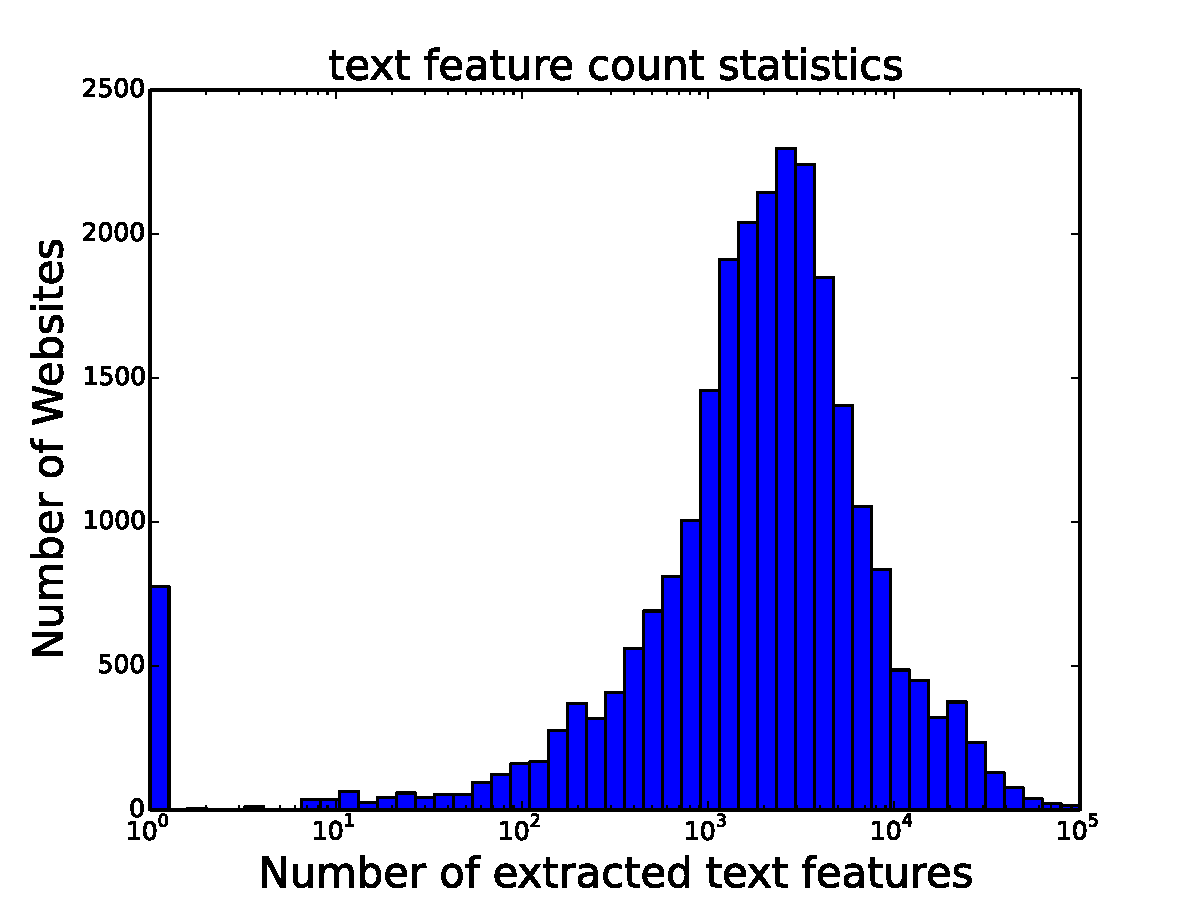
\includegraphics[width=.45\textwidth]{fig/text-feature-stats}
    \label{fig:text-feature-stats}
  }
  \subfigure[]{
    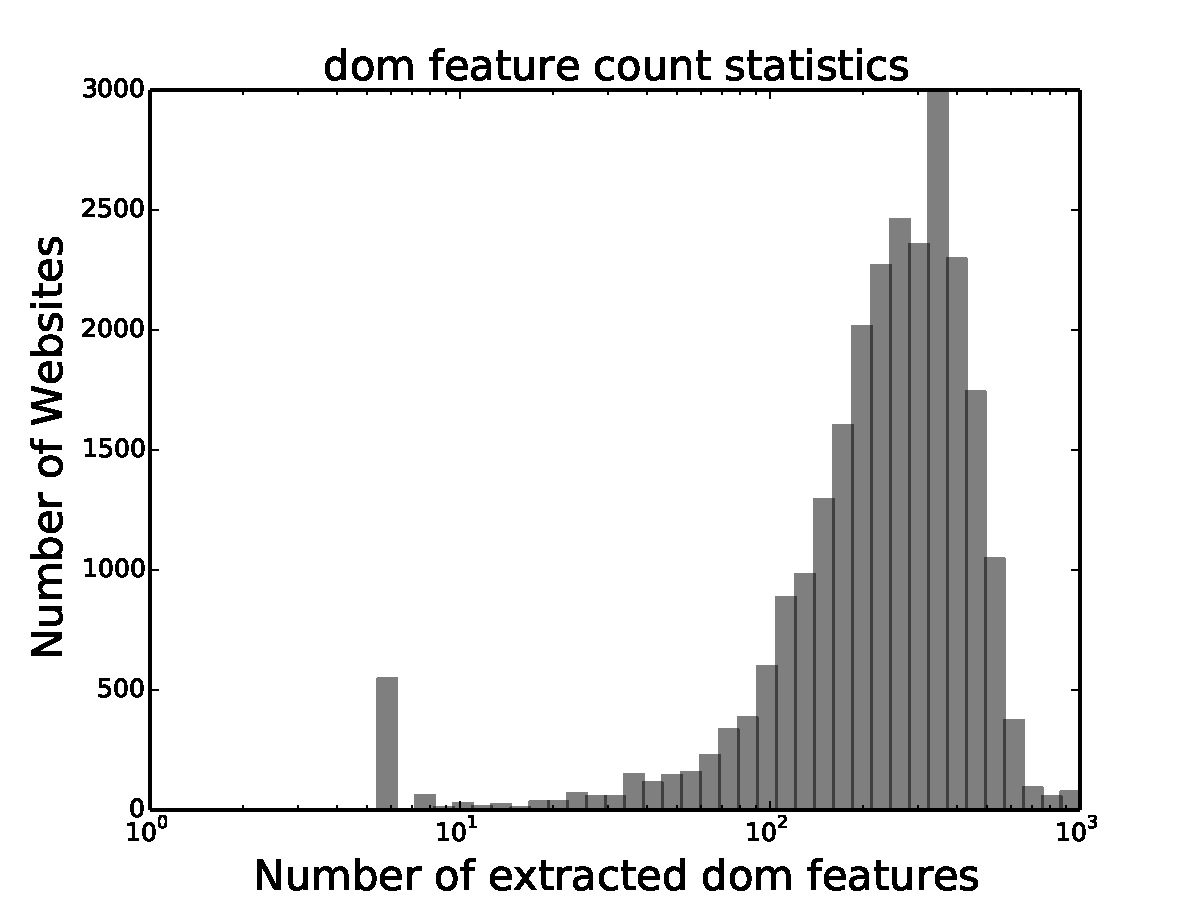
\includegraphics[width=.45\textwidth]{fig/dom-feature-stats}
    \label{fig:dom-feature-stats}
  }
  \caption{Number of text and dom features extracted from different websites}
\end{figure*}

In order to detect cloaking, we need to capture the bahavior and similarity that
a same website maintains. Inspired by ~\cite{wang2011cloak}, this work looks at
both text and dom features and generate simhash separately.
%We implemented the text-simhash algorithm 
%same as the simhash algorithm used in spam detection by Google.
%described
%in ~\cite{manku2007detecting},

For text simhahsh, the algorithm extracts visible sequence of words from website.
From the sequence, this algorithm extracts words, bi-gram, tri-gram set
(repeated elements only recorded once). For example, for
sentence: thank you so much, corresponds to feature set \{thank, you, so, much,
thank you, you so, so much, thank you so, you so much\}.
Because there are usually large number of words on a website, Requirement (B)
suffices. ~\autoref{fig:text-feature-stats} shows text feature statistics on %25610 urls in
urls obtained from hot search results $D_{hot, search}$. Since bi-gram, tri-gram 
shows how words are concatenated and represents strcture of documents,
Requirement (A) suffices. This algorithm is used rather than weighted version
described in  ~\cite{manku2007detecting}, because it is light-weight and doesn't
require inverse document frequency and phrase detection. This is important
in our case, because we are designing an algorithm that is deployable in user
browser, where efficiency matters.
%text feature set
%We implemented the text-simhash algorithm 
%same as the simhash algorithm used in spam detection by Google.
%described
%in ~\cite{manku2007detecting},

%and has great benefit in our use scenario, because this requires a single pass
%of the document and no extra information. In contrast,
%~\cite{manku2007detecting} implement extract weighted features using standard IR
%techniques like tokenization, case folding, stop-word removal, stemming and
%phrase detection, and may introduce more overhead and need extra knowledge.

\begin{figure}[t]
  \centering
  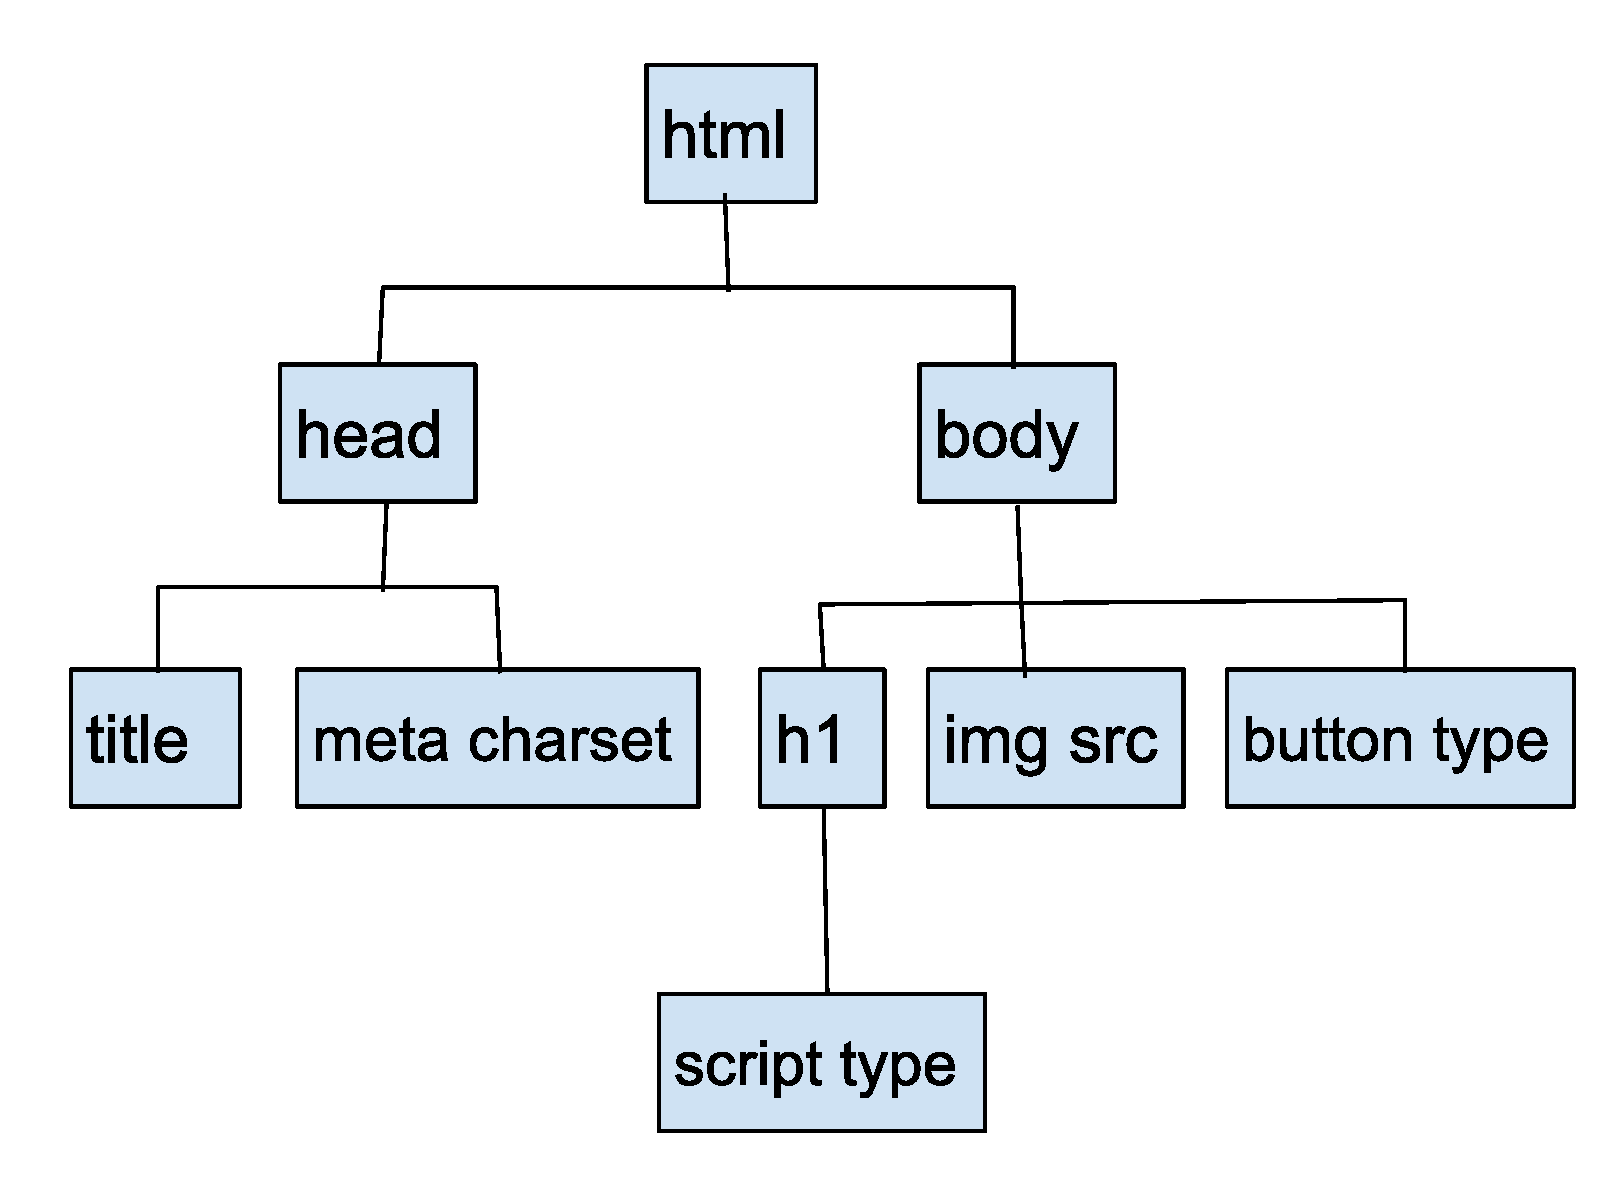
\includegraphics[width=.5\textwidth]{fig/dom-tree}
  \caption{DOM tree example}
  \label{fig:dom-tree}
\end{figure}

Regarding structure of websites, we design an algorithm to extract DOM features
out of DOM tree.

For each DOM tree, we record presence of each node (tag name), as
well as presence of each child parent pair. The node set tells us information about what
tag is present in this page, and child parent pair tells us how these tags are
organized, i.e., structure information, suffices Requirement (A).
Since we are recording presence of tags and type of tags are relatively small,
we record tag name and associated attribute names to gain more features (higher
entropy).
Attribute value is discarded because based on our observation, attribute value
may change on every visit.
For example,
~\autoref{fig:dom-tree} correspond to feature set 
\{html, head, body, title, \ldots, (head, html), (body, html), \ldots \}
%\{html, head, body, title,
%  meta charset, h1, img src, button type, script type, (head, html), (body,
%  html), (title, head), (meta charset, head), (h1, body), (img src, body),
%(button type, body), (script type, h1)\}

~\autoref{fig:dom-feature-stats} shows dom
feature statistics $D_{hot, search}$ and the number of features extracted in this
fashion is relatively large, suffices Requirement (B). 


% you can also use the wonderful epsfig package...
\begin{figure}[t]
  \centering
  \subfigure[User View of Yahoo Text Simhash]{
    \centering
    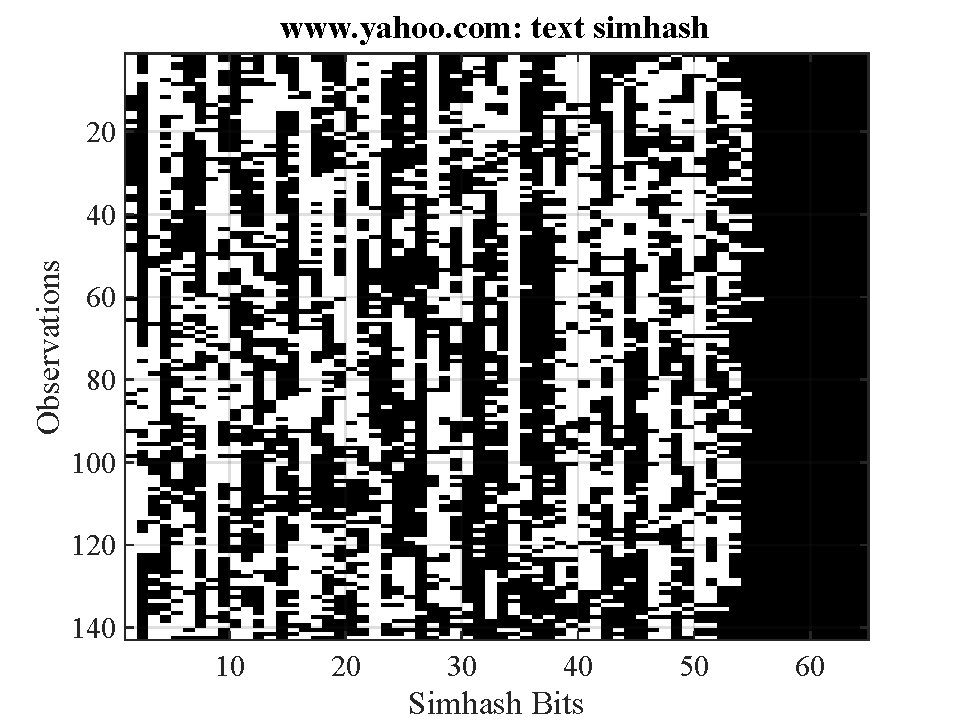
\includegraphics[width=.5\textwidth]{fig/yahoo-text-user}
    \label{fig:yahoo-text-user}
  }
  \subfigure[User View of Yahoo DOM Simhash]{
    \centering
    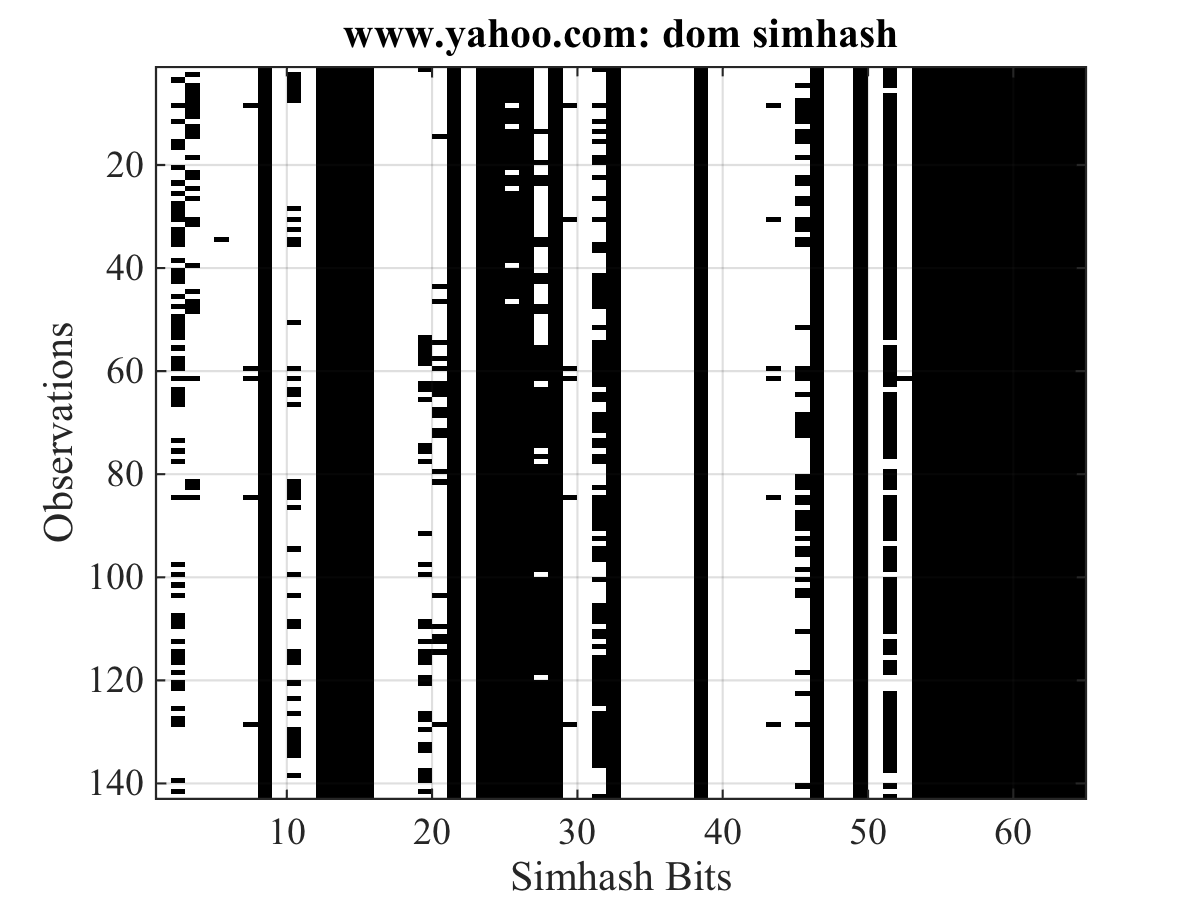
\includegraphics[width=.5\textwidth]{fig/yahoo-dom-user}
    \label{fig:yahoo-dom-user}
  }
  \caption{Yahoo simhash changes over 7x24 period Feb.1-7, 2015}
  \label{fig:yahoo-simhash}
\end{figure}

~\autoref{fig:yahoo-simhash} gives an example on how DOM and text simhash looks
like and how they are distributed on {\it www.yahoo.com} over 7 x 24 period from
Feb.1, 2015 to Feb.7, 2015. ~\autoref{fig:yahoo-text-user} shows text simhash
and ~\autoref{fig:yahoo-dom-user} shows dom simhash. The x-axis is bits of simhash value and
y-axis is the id of each observation (id increases in the order of collection time).

It is pretty straightforward from ~\autoref{fig:yahoo-simhash} that,
text simhash changes rapidly, indicating dynamic nature of this
website, and dom simhash changes relatively slow and less.

Till now, we have demonstrated the algorithm we are using to generate
text-simhash and dom-simhash out of a website. Based on our observation, the
text-simhash might change rapidly, while dom-simhash relatively remain the same.

\subsubsection{Clustering}
\label{sss:clustering}
Websites could have multiple versions of content due to many reasons.
An example is page construction. The server might return some notice or help
information for apology and instructions on what to do next.
Since we are monitoring websites over a period of time, we need to be able to
build model for different version of websites and learn corresponding pattern.

Different from ~\cite{manku2007detecting}, we not only want to know whether two pages are
duplicate, we also want to know the patterns of these simhash. In this work, we employ
hierarchical clustering to do this job.

Since simhash maps a high-dimensional
features set into fixed number of bits, where hamming distance represents the
similarity between the original feature set. We leverage the fact that hamming
distance is euclidean distance (L1 norm on 64 dimension). On each dimension, the
original value is either 0 or 1. But it can be averaged and centriod can be
computed.

In this work, we use agglomerative hierarchical clustering ~\cite{jones2014scipy} to cluster
collected simhash. This is a bottom up approach: each observation starts in its
own cluster, and pairs of clusters are merged as one moves up the hierarchy.
In order to decide which clusters should be combined, a measure of dissimilarity
between sets of observations is required. In most methods of hierarchical
clustering, this is achieved by use of an appropriate metric (a measure of
distance between pairs of observations), and a linkage criterion which specifies
the dissimilarity of sets as a function of the pairwise distances of
observations in the sets. This work represents each simhash as a 64 dimension
bit vector and specifies hamming distance as distance metric. The linkage method
used is average distance and criterion is inconsistent coefficient.

%These choices are reasonable. 
{\bf Average linkage:} 
Consider the following use case, spider collect
multiple copies of a website and compute corresponding simhash $S_{spider} = \{s_{i}, i \in
(1,n)\}$ and the user return observation $s_{user}$ for this website. In order to
compare $s_{user}$ with $S_{spider}$, and take into consideration of the all the
collected simhash, the distance from $s_{user}$ to centroid of $S_{spider}$ is a
reasonable measure. In order to be consistent with detection phase (user versus
spider), clustering phase uses average linkage as well.

{\bf Inconsistency coefficient:} this coefficient characterizes each link in a cluster tree by
comparing its height with the average height of neighboring links at the same
level and below it in the tree. The higher the value of this
coefficient, the less similar the
objects connected by the link. By using threshold of inconsistency
coefficient as criterion, we could get several clusters for each website.

\begin{equation}
  \label{coefficient:define}
  \alpha  = \frac{d - \mu}{\sigma}
\end{equation}

~\autoref{coefficient:define} explains how inconsistent coefficient is computed.
$\alpha$ is inconsistent coefficient, $d$ is the distance between two
clusters, $\mu$ is mean of the heights of all the links included in the
calculation, $\sigma$ is standard deviation of the heights of all the links
included in the calculation. In our case, each computation includes all links at
the same level and below it, and this is done by setting $depth$ in
$inconsistent(Z, depth)$ ~\cite{icintro} to $m-1$, where $m$ is total number of observations.

\begin{equation}
  \label{coefficient:learn}
  \begin{gathered}
    S_{spider, r} = \{centroid_r, links_r\}, \\
    S_{spider, s} = \{centroid_s, links_s\} \\
    \alpha = \frac{d_{r,s} - \mu}{\sigma}, \text{merge } S_{spider, r},
    S_{spider, s} \text{ if } \alpha < T_{learn} \\
    d_{r, s} = \frac{1}{n_rn_s}\sum_{i=1}^{n_r}\sum_{j=1}^{n_s} dist(s_{spider,
    r, i}, s_{spider, s, j}) \\ 
    \mu = avg(x), x \in  links_i \cup links_j \\
    \sigma = std(x), x \in link_i \cup links_j \\
  \end{gathered}
\end{equation}

Let $T_{learn}$ denote the threshold for inconsistent coefficient, 
~\autoref{coefficient:learn} shows the merging criterion in clustering phase.
After clustering, $S_{spider}$ is divided into $c$ clusters $S_{spider, k}, k \in (1, c)$.
These clusters are Simhash-based Website Model for this website.

We denote each cluster $S_{spider, k}$ with centroid and links formed in
clustering phase $S_{spider, k} = \{centroid, links\}$. This representation is
intended for comparison with a new observation (single node cluster). $centroid$ is used to
compute distance from new observation to current cluster, $links$ are used
to compute $\mu$ and $\sigma$.

%For different websites, simhash can be considered as an algorithm to map them to
%a 64-bit number randomly ~\cite{manku2007detecting}. For the same website,
%simhash measures the similarity between them.
%



%In order to decide the number of clusters to take in hierarchical clustering
%(when to stop), we use inconsistent coefficient.
%
%considerations of significance, we ask whether this is an unusual result or
%whether it could have arisen merely by chance
%
%One way to determine the natural cluster divisions in a data set is to 
%linkage metric: hammming
%method: Unweighted average distance (UPGMA)
%cutoff: inconsistent value less than c
%pick inconsistent value now!!!!!
%


%\begin{gather*} \label{npa}
%  d(u,v) = \min(dist(u[i],v[j])) \\
%  \text{for all points i in cluster u and j in
%  cluster v. }
%\end{gather*}
%This~\autoref{npa} is known as the Nearest Point Algorithm.
%
%Single-linkage clustering is one of several methods of agglomerative
%hierarchical clustering. In the beginning of the process, each element is in a
%cluster of its own. The clusters are then sequentially combined into larger
%clusters, until all elements end up being in the same cluster. The stop
%criterion is the distance one.

\subsection{Cloaking Detection}
In the above section, for observations of each website, $S_{spider}$, we have 
learned clusters , which is $S_{spider, k}, k \in (1, c)$. For each cluster, we
represent it as $S_{spider, k} = \{centroid, links\}$.
In order to use these clusters, we first illustrate how the comparison can be
done.

In order to detect SEO and SEM cloaking,
this work first search and click results with normal user agent, then visit 
landing urls collected with google bot user agent (described in detail in
~\autoref{ss:dataset}).
For a specific website, we denote user observation of this website as
$s_{user}$, denote spider copies as $S_{spider}$ and 
$S_{spider, k}$ are the learned clusters.

For each cluster $S_{spider, k}$, we record link heights and centroid.
When comparing $s_{user}$ with $S_{spider, k} = \{centroid, links\}$, 
distance $d'$ from $s_{user}$ to $centroid$ is computed, which is average distance
from cluster $\{s_{user}\}$ to $S_{spider, k}$. In ~\autoref{sss:clustering}, we
merge clusters if inconsistent coefficient $\alpha < T_{learn}$. Similarly, we
could compute inconsistent coefficient $\alpha'$ for $\{s_{user}\}$ to $S_{spider, k}$ as
shown in ~\autoref{coefficient:detect} and use detection threshold to reject
$s_{user}$.

\begin{equation}
  \label{coefficient:detect}
  \begin{gathered}
    \text {If } \alpha' = \frac{d' - \mu}{\sigma} > T_{detect}, \text{reject } s_{user} \\
    d' = \frac{1}{n_k}\sum_{i=1}^{n_k} dist(s_{user}, s_{spider, k, i}) =
    dist(s_{user}, ceontroid) \\ 
    \mu = avg(x), x \in  \{d'\} \cup links \\
    \sigma = std(x), x \in \{d'\} \cup links \\
  \end{gathered}
\end{equation}

For observation $s_{user}$, if all clusters $S_{spider, k}, k \in (1, c)$ rejects it, then
mark $s_{user}$ as cloaking.

\begin{figure}[t]
  \centering
  \subfigure[User View of Google Dom Simhash]{
    \centering
    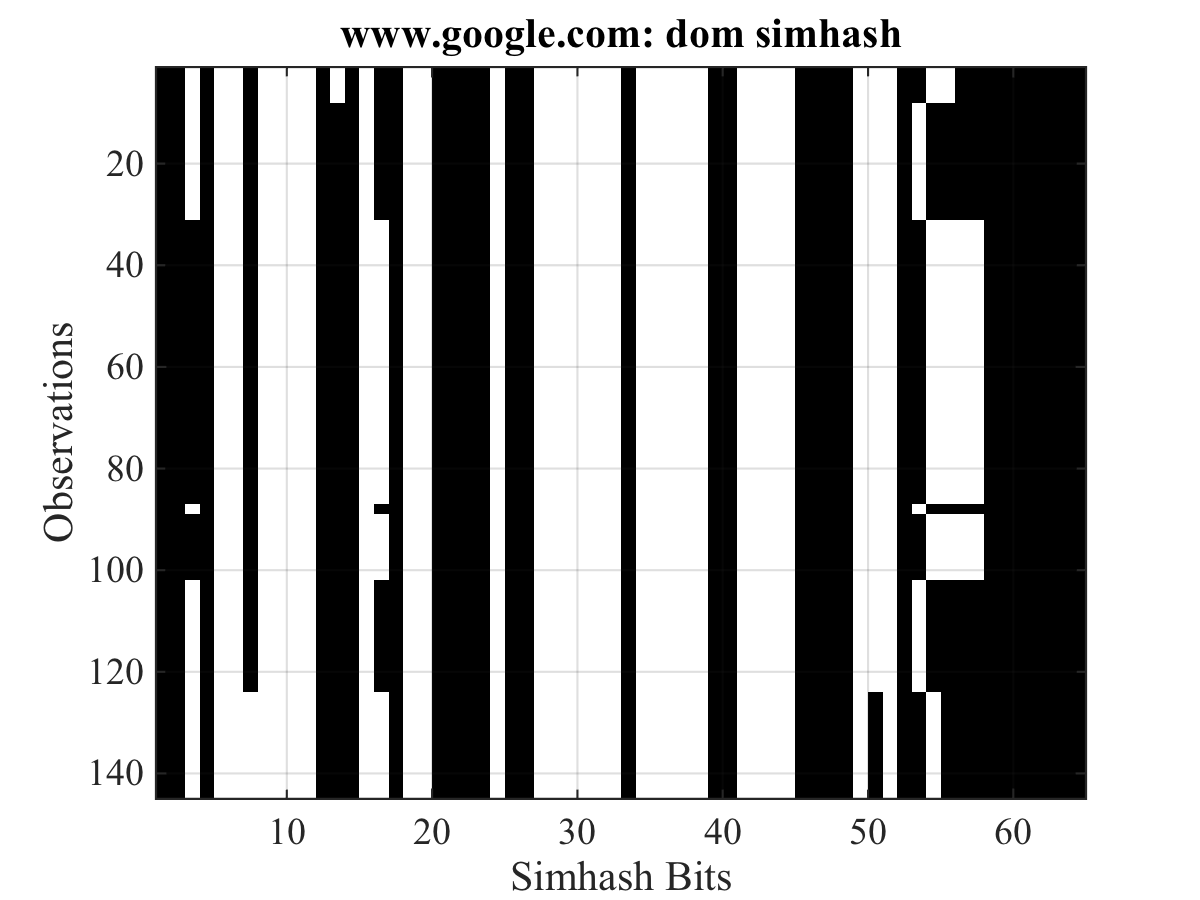
\includegraphics[width=.5\textwidth]{fig/google-dom-user}
    \label{fig:google-dom-user}
  }
  \subfigure[Spider View of Google Dom Simhash]{
    \centering
    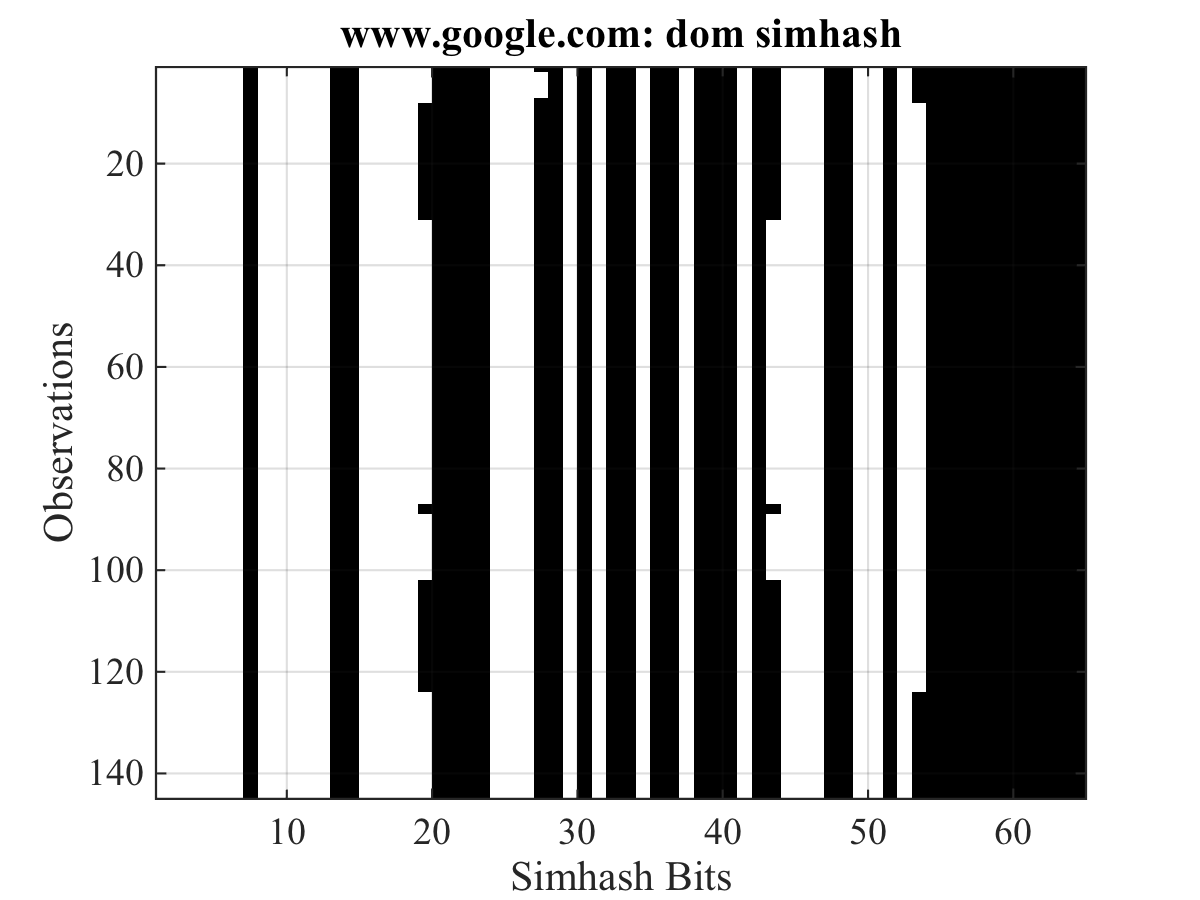
\includegraphics[width=.5\textwidth]{fig/google-dom-google}
    \label{fig:google-dom-google}
  }
  \caption{Comparison of user and spider copies dom simhash, over 7x24 period Feb.1-7, 2015}
  \label{fig:google-simhash}
\end{figure}

However, in reality, there can be consistent differences between what spider
sees and what user sees and this is totally leagal. For example, a website
delivers non-javascript version to spider, but javascript version to user.
~\autoref{fig:google-simhash} shows the difference between spider and user
observations of {\it www.google.com} DOM simhash. Another example is that a website may
present advertisements to normal user, but non-advertisement version to spider.
Besides, there are websites that rarely changes at all, meaning $\sigma$ is
zero, thus ~\autoref{coefficient:detect} doesn't work. To fix the two problems, we introduce
a minimum radius $R_{detect}$. The modified formula is ~\autoref{radius:detect}:
\begin{equation}
  \label{radius:detect}
  \text{If } d' - R_{detect} - \mu > T_{detect} \sigma, \text{reject } s_{user}
\end{equation}

~\label{s:evaluation} evaluates the proposed SWM and cloaking detection
algorithm, and provides insights and suggestion on selection of $T_{learn}, T_{detect},
R_{detect}$.

%Classification hinges on having access to a robust set of features derived from
%URLs to discern between spam and non-spam. Previous work has shown that lexical
%properties of URLs, page content, and hosting properties of domains are all
%effective routes for classification [15], [16], [22]–[24]. We expand upon these
%ideas, adding our own sources of features collected by one of three components:
%a web browser, a DNS resolver, and IP address analysis. A comprehensive list of
%features and the component that collects them can be found in Table 1. A single
%monitor oversees multiple copies of each component to aggregate results and
%restart failed processes. In turn, the monitor and feature collection components
%are bundled into a crawling instance and replicated in the cloud


%\subsection{Model Selection}
%
%
%\begin{table*}[!th]                                                     
%  \centering                                                            
%  \scriptsize                                                           
%  \begin{tabular}{lllllllllll}
  \toprule
  & \multicolumn{2}{c}{\textbf{Normal}}
  & \multicolumn{2}{c}{\textbf{Lognormal}}
  & \multicolumn{2}{c}{\textbf{Exponential}}
  & \multicolumn{2}{c}{\textbf{Gamma}}
  & \multicolumn{2}{c}{\textbf{Logistic}}\\

  \textbf{Website(Hash Type)\textbackslash Model}
  & AD-value
  & P-value
  & AD-value
  & P-value
  & AD-value
  & P-value
  & AD-value
  & P-value
  & AD-value
  & P-value \\
  \midrule
  digg.com T & 0.617 &  0.100 & 0.481 &  0.219 &
  14.851 & < 0.003 & 0.538 &  0.186 & 0.531 &  0.131\\ 
  digg.com T & 0.227 &  0.806 & 0.179 &  0.914 &
  19.690 &  < 0.003 & 0.198 &  > 0.250 & 0.250 & >0.250\\
  yahoo.com T & 0.192 &  0.893 & 0.263 &  0.692 &
  35.828 & <0.003 &   0.231 & >0.250 & 0.222 & >0.250\\
  amazon.com T & 0.720 &  0.058 & 0.323 &  0.520 & 
  27.754 & <0.003 &  0.436 & >0.250 & 0.642 &  0.058\\
  reddit.com T & 0.373 &  0.411 & 0.331  & 0.509 & 
  35.063 & <0.003 & 0.340 & >0.250 & 0.361 & >0.250\\
  yacombinator.com T & 0.473 &  0.237 & 0.516 &  0.186 &
  37.551 & <0.003 & 0.519 &  0.204 & 0.583 &  0.089\\

  digg.com D & 0.319 &  0.372 & 0.348 &  0.305 &
  1.491 &  0.021 &  0.402 & >0.250 & 0.363 & >0.250\\
  yahoo.com D & 0.531 &  0.168 & 0.392 &  0.366 &
  18.837 & <0.003 & 0.441 & >0.250 & 0.584  & 0.088\\
  amazon.com D & 1.519 & <0.005 & 0.916 &  0.019 &
  22.083 & <0.003 & 1.052 &  0.009 & 0.548 &  0.114\\
  amazon.com D & 0.483 & 0.117 &  0.504 & 0.104 &
  1.741 & 0.010 & 0.601 & 0.128 & 0.523 & 0.115\\

\end{tabular}

                                     
%  \caption{Model statistics for selected websites}
%  \label{tbl:para-select}                                         
%\end{table*}                                                            
%
%
%This table ~\autoref{tbl:para-select} shows the Anderson-Darling (AD) value and P-value for each model.
%A common rule used in model selection is pick the model which has the smallest
%value with P-value greater than 5\%. Each row in the table represents one
%website. From the statistics of these websites, we choose normal distribution
%for text simhash and Lognomal distribution for dom simhash.
%
%In the simhash based cloaking detection model, input from the user is simply simhash. How to compare against the simhashs that is already collected?
%
%One simple way is to compute the average distance from this simhash to all the observed simhashs. The next step is then to tell whether this distance is reasonable. 
%
%The text distribution follows lognormal distribution.
%After mannual check of those results.
%
%

\subsection{Dataset}
\label{ss:dataset}
This work is focusing on detecting cloaking in SEO and SEM, therefore, we
collect search words for both SEO and SEM.

\subsubsection{Keywords}
Similar to ~\cite{wang2011cloak},
in order to detect and measure cloaking that intended to gather high volumes of
undifferentiated traffic, and those target on specific cloak search terms, we
collected two set of words, hot search words $W_{hot, search}$ and abuse
oriented words $W_{spam, search}$. $W_{hot, search}$ consists of 170
unique monthly hot search words
from Google trend ~\cite{google-trend} from Jan 2013 to Dec 2014. $W_{spam,
search}$ is first manually collected by referring to ~\cite{google-ad-policy} for
basic abuse oriented words in search engine, mainly from categories including
gaming ad network, adult-oriented content, alcoholic beverages,
dangerous products, dishonest behavior,
gambling-related content, healthcare and medicines. Then we expand $W_{spam,
search}$ using Google Suggest, and get 1024 words.

For SEM cloaking detection, the selection of keywords is a different, because
Google Adwords system is based on a real time bidding system and advertisers will bid on
monetizable keywords, e.g. instant loan, but not on navigational keywords, e.g.
facebook. Inspired from ~\cite{chellapilla2006improving}, we
collect monetizable words for advertisement collection. Monetizability is
measured by Google Keyword Planner (GKP) ~\cite{keyword-planner}. Keyword planner
provides convenient API for checking competition and suggested bid for list of
keywords. Similar to SEO, we collect monetizable keywords from hot search and
abuse oriented list. Abuse oriented ad words are collected by filtering words
that has no competition and no bid price in $W_{spam, search}$, as a result, 573
words composes spammy advertisement word set $W_{spam, ad}$. In order to get as
much advertisements as possible, we collect 11671 hot keywords from Google Trend
~\cite{google-trend} (from 2004 to 2014, and each categories are collected), 
filter this word set by GKP, and get 4108 keywords, $W_{hot, ad}$.

%9 cat: 686
%dishonest: 103
%
%gambling: 128
%dangerous: 64
%health: 43


%We have collected four datasets, spammy search, $D_{spam, search}$, hot search,
%$D_{hot, search}$, spammy ads $D_{spam, ad}$, hot ads, $D_{hot, ad}$. 
%$D_{spam, search}$, spammy search words collected manually, \XXX{N} words.
%$D_{hot, search}$, hot search monthly words from Jan 2013, Dec, 2014, 24 month
%in total,  \XXX{N} words.
%From $D_{hot, search}$, we evaluate the monetizability of each word through
%Google Keyword Planner~\cite{keyword-planner} and simply
%remove the words that have no bid price. This results in our spammy
%advertisements words set, $D_{spam, ad}$, we have collected advertisements from 573 words.
%$D_{hot, ad}$, we need as much words as possible, i.e. as much ads as possible,
%therefore first download hots words list from Google Trend, for hot words in
%each category, we download weekly, monthly, and yearly from 2004 to 2014, and
%then we find the useful keywords with Keyword Planner~\cite{keyword-planner}.
%We have collected advertisements from 4108 words.
%

%
%Because we want to measure cloaking in SEO and SEM, we have compiled a list of
%cloaking words, from the policies specified by Adwords, inspired by the words
%collection process in ~\cite{wang2011cloak}. We have looked at the policies, and
%collected \XXX{N} words, from ad network abuse, adult abuse, alcohol abusive, dangerous behavior
%abuse, dishonest behavior abuse, health abuse, gambling abuse.
%

\subsubsection{Crawling}
\label{sss:crawling}
Starting from the four collected keyword set, we automate browser to do
search-and-click. This work uses Selenium ~\cite{selenium}, an open source
browser automation tool, to visit websites while mimicked as users and spiders.
For SEO keywords crawling, we set browser user agent to 

{\it Googlebot/2.1
(+http://www.google.com/bot.html)}

to mimic Google bot and 

{\it Mozilla/5.0 (Windows NT 6.3; Win64; x64) AppleWebKit/537.36 (KHTML, like
Gecko) Chrome/37.0.2049.0 Safari/537.36}

to mimic Chrome user on windows
machine. For SEM keywords, Chrome user setting is the same, but spider user
agent is set to {\it AdsBot-Google (+http://www.google.com/adsbot.html)}, which
is the user agent used by Google to inspect ads and advertisement landing pages
are required by Adwords Policy ~\cite{google-ad-policy} to show consistent 
content to Google and normal user.

In SEO, we use a university IP running ubuntu to perform crawling (browser user
agent can be forged, thus will be considered as windows machine by site owner).
Since redirection is popular on Internet, what user actually clicks may not be
where he goes to. In this work, we denote the link that user directly clicks on
or input to browser as $URL_{visit}$, and resulting page that user is finally
led to as $URL_{landing}$.
The crawling process is: 
(A) For each word in $W_{hot, search}$ and $W_{spam, search}$, we search in Google
and click on top 200 result as normal user. The landing url $URL_{landing, user}$ 
and website content are saved to disk. 
(B) For landing urls collected in step (A), we directly visit them 6 times
(because we need multiple spider copies to learn clusters) as Googlebot and
save website content and record the landing url in step (A), $URL_{visit,
spider} = URL_{landing, user}$.

The above steps are different from past approaches ~\cite{lin2009detection,
wu2005cloaking, wang2011cloak}, which visit $URL_{visit, user}$ in step (B). Our
approach is reasonable, because we leverage the fact that, in order to reach
real user, $URL_{landing, user}$ have to show cloaked content to user. If 
site owner cloaks on landing page, we can catch them; and if site owner employs
redirect cloaking~\cite{wu2005cloaking}, he has the incentive to cloak on
landing page in order to evade inspection.

In SEM, the crawling process is similar, except that: word sets are
$W_{hot, ad}$ and $W_{spam, ad}$; click and visit ads in fist 5 pages as normal
user (empirically only first 5 pages contains advertisemetns); 
and spider user agent is set to ads bot.

\subsubsection{Data Statistics}
Through steps described in ~\autoref{sss:crawling}, we get four datasets,
$D_{spam, search}$, $D_{hot, serch}$, $D_{spam, ad}$ and $D_{hot, ad}$.
Since we are modeling website on a per url basis and parameters in url may
change every time of visit, it is necessary to define the granularity of
comparison. For simplicity, we strip all the parameter
values and keep all the parameter names, and throw away the scheme field, i.e.
{\it http://www.gatech.edu/?user=1234} is simplified to
{\it //www.gatech.edu/?user=}. Under this definition of url, $D_{spam, search}$
has 129393 unique urls, $D_{hot, search}$ has 25533, $D_{spam, ad}$ has 2219,
and $D_{hot, ad}$ has 25209 
\footnote{Automating website visit through selenium
  and chrome can sometimes result in rendering errors or empty content, these
examples are removed from collected dataset}.


%\subsection{Server-based Cloaking Detection System}
%The server based detection system.
%For each search word, user visit once, then spider visit 6 times (this number
%can be tweaked) and we levearge the fact that, if we want to monitor the change
%of a website, multiple copies are essential.
%



\section{Evaluation}
\label{s:evaluation}


%1. Collect terms
%2. Query search results.
%3. Crawl data and get ground truth (how
%many).
%4. Train model and select parameters use 5-fold stratified cross validation
%~\cite{scikit-learn}.

In the above section ~\autoref{s:methodology}, we propose the SWM and explains
how it can be used to do cloaking detection (outlier detection). There are three
parameters to be learned, the upper bound of inconsistent coefficient in
learning phase $T_{learn}$, the lower bound of inconsistent coefficient in the detection
phase $T_{detect}$, the fix parameter minimum radius $R_{detect}$. 
There are four dataset collected in ~\autoref{s:methodology}. In this section,
we first describe the groundtruth obtained from $D_{spam, search}$ and $D_{hot,
search}$. Then train and test the performance of the proposed model.

\subsection{Groundtruth}

%We randomly sample 600 websites from the dataset, for 10 times. This results in
%5726 websites. We manually label them and \XXX{cloaking}, \XXX{not}, percentage
%for each is.
Similar to ~\cite{lin2009detection}, we first remove duplicates (same simhash
from user side and Google side), then label $D_{spam, search}$ and $D_{hot,
search}$. We also manually add the examples that we observe when we do case
study. We manually labeled 1195 cloaking examples. And we randomly
 5308 samples from non-cloaking dataset. This composes our
dataset 6503 for algorithm learning.

%\subsubsection{De-duplication}
%71116 urls
%
%62042 websites
%
%This results in \XXX{Some} links. Then we compare the text simhash and dom
%simhash, remove those which are exactly duplicate of one of the simhash observed
%by Google. After this step, we have \XXX{N} url left.
%
%For advertisements, after deduplication, there are 997 (score 60) urls remained.
%
%For search results, after deduplication 37155 urls, 35444 websites remained.



%We remove the failure websites and this results in 
%113242 urls, exact match, parameter different are counted.
%98390 sites, parameters ignored. Later we will use the latter parameter because
%it makes more sense.

%Step 1: Filter
%
%In order to get groundtruth, we follow a similar process employed in
%~\cite{lin2009detection}, we first filter the results and get rid of the highly reputated ones. We write a
%script to query the WOT API, and remove websites with combined score 80
%(which is a pretty high score) and the results are \XXX{N} urls after that.
%
%for advertisements, after filtering, there are 2279 (score 60) urls
%remained.\XXX{Problematic because I haven't merged them}
%
%for search results, after filtering, there are 90120 (60) urls remained.
%\XXX{Problematic because I haven't merged them}
%

%\subsubsection{Random Sample and Labeling}
%Then we randomly select 1000 urls from the dataset, and label them, after
%labeling, we found \XXX{N} cloaking sites and \XXX{M} dynamic websites.
%These are the groundtruth we used to label our data.


\subsection{Detection and Evaluation}

\subsubsection{Selection of $T_{learn}$ and $T_{detect}$}
Because $R_{detect}$ is a parameter to allow the system to handle consistent
difference between spider and user copies, therefore, we first set detect
$R_{detect}$ to be zero, do 5 fold stratified cross validation~\cite{scikit-learn}.
on the result. 
In the learning phase,
Our objective function is to first minimize the total number of errors in classification $E = FP + FN$, and
if $E$ is the same, minimize $d = T_{detect} - T_{learn}$.
This is reasonable because $d$ is the area that we cannot judge, and the smaller
the area, indicates that the learned model is more compact. The two objective
function are widely used metrics in machine
learning parameter selection \XXX{cite}.

By applying five-fold cross validation on the groundtruth, and the described
objective function, dom simhash returned 
$T_{detect, dom} = 1.8$ and $T_{learn, dom} = 0.7$, and text simhash yields
$T_{detect, text} = 2.1$ and $T_{learn, text} = 0.7$.
% this is meaningless, i think
%
% majority is false positive.
% which yields to distance 1.1 at optimal (1318.4 learn error, 329 detect error), 
\subsubsection{Radius Selection $R_{detect}$}
From the above section, we have selected $T_{detect, dom} = 1.8$ and $T_{learn, dom} = 0.7$,
$T_{detect, text} = 2.1$ and $T_{learn, text} = 0.7$. Now, we want to decide,
$R_{detect, text}$ and $R_{detect, dom}$ separately. In this section, we conduct
three experiments: cloaking detection using (1) dom simhash (2) text simhash (3)
both dom simhash and text simhash.
Again, we use five-fold cross validation to learn and test the dataset. The
selected parameter for dom simhash is $R_{detect, dom} = 17$, text simhash is
$R_{detect, text} = 16$. If we consider great difference in both text and dom as
cloaking (intersect the detected results), the result is $R_{detect, dom} = 13$,
$R_{detect, text} = 17$, get $FPR = 0.1\%, TPR = 94\%$.
~\autoref{fig:roc} gives an illustration on how FPR and TPR changes as
threshold for DOM and TEXT changes.

% you can also use the wonderful epsfig package...
\begin{figure}[t]
  \centering
  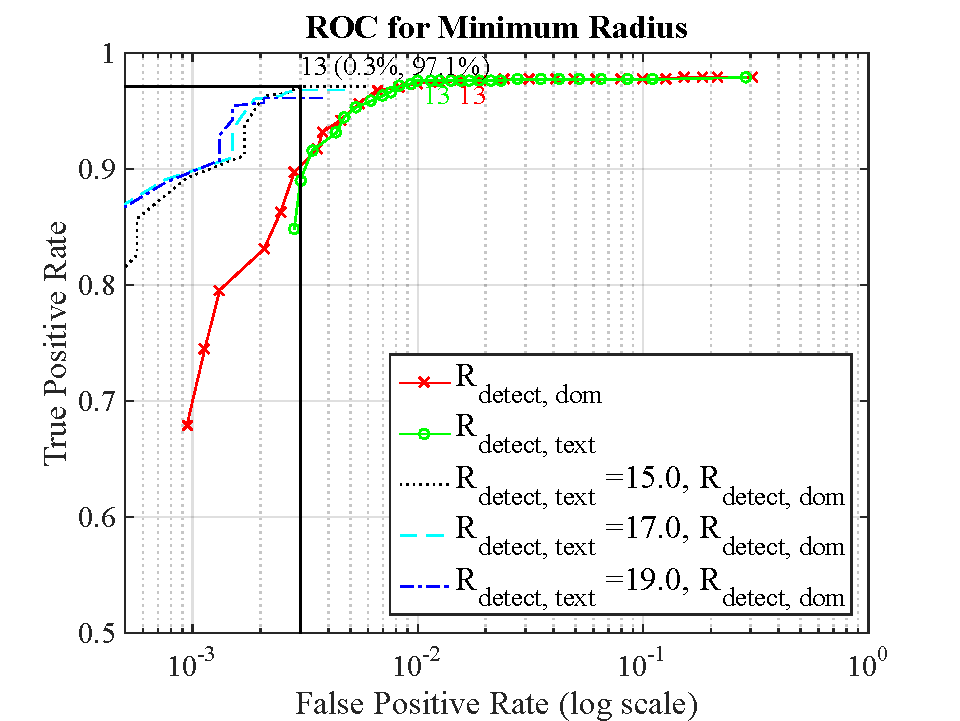
\includegraphics[width=.5\textwidth]{fig/roc}
  \caption{ROC for DOM, TEXT, DOM \& TEXT}
  \label{fig:roc}
\end{figure}

With the learned model, in Section ~\autoref{s:measurement} 
detect on the four dataset that we obtained and
manually label the results. In our detection, we want a low false positive rate,
therefore, we use the FPR = 0.1\%, TRP = 92\% in ~\autoref{fig:roc}. This yields
to $R_{detect, dom} = 16$, $R_{detect, text} = 20$.


\subsection{Efficiency Comparison}
\label{ss:efficiency}
While we can achieve similar false positve rate and true positive rate compared
to past approaches, we argue that, our approach is much more efficient than past
approaches and is light-weight enough to be deployed on user browser.
\XXX{Table} is a comparison of time complexity and number of rounds that the
documents need to be processed (each time they get smaller amount of document,
though). Let $N$ denote the number of total urls collected, $M$ denoete the
number of cloaking websites. The time complexity is \XXX{Plot}.



For simhash computation, we implements a browser extension which exposes
negligible overhead to user. We 

\XXX{the table comparing our approach with past cloaking detection approaches}
\XXX{the ability of simhash in measuring difference}.






\section{Measurement}
\label{s:measurement}

With the model built in ~\autoref{s:evaluation}, we detect cloaking in
the four collected datasets, spammy search, $D_{spam, search}$, hot search,
$D_{hot, search}$, spammy ads $D_{spam, ad}$, hot ads, $D_{hot, ad}$. 
$D_{spam, search}$. From our observations, we categorize cloaking websites into 9 types:
pharmacy, gambling, loan, general traffic sale, pay per click, error page, illegal service,
phishing, bad domain and malware downloading. To better analyze cloaking incentives, 
we divided traffic sale into 4 categories: pharmacy, gambling, loan and general traffic sale. 


In SEO field, we detect cloaking websites in spammy search and hot search field. In spammy search,
we applied our cloaking detection system on 129393 websites. Cloaking detection system reported 2491
cloaking websites. 661 websites are cloaking of pharmacy. 1514 websites are cloaking of gambling.
33 websites are cloaking of loan. 28 websites are cloaking of general traffic sale. 28 websites are cloaking
of pay per click. 43 websites are cloaking of error page. 122 websites are cloaking of illegal service. 
17 websites are cloaking of phishing. 73 websites are cloaking of baddomain. 20 websites are cloaking of malware downloading.
In hot search, we applied our cloaking detection system on 25533 websites. Cloaking detection system reported 93
cloaking websites. 33 websites are cloaking of pharmacy. 2 websites are cloaking of gambling.
26 websites are cloaking of loan. 27 websites are cloaking of traffic sale. 2 websites are cloaking of cloaking of
error page. 2 websites are cloaking of illegal service. 3 websites are cloaking of bad domain. 

In SEM field, we deteck cloaking websites in spammy ads and hot ads. In spammy ads,
we applied cloaking detection system on 25533 websites. Cloaking detection system reported 6 cloaking websites.
1 website is cloaking of pay per click. In hot ads, we applied cloaking tection system on 25209 websites.
Cloaking detection system reported 10 cloaking websites. 4 websites are cloaking of traffic sale.
6 websites are cloaking of illegal service. 



\subsection{Cloaking in SEO}

SEO: How severe is cloaking? How many categories and percentages of various
cloaking? For each type of cloaking, what are their incentives?

\XXX{Plot a log scale pie or histogram for categories in SEO}
Out of the 20k distinct urls, we detect 1600 urls. There are mainly composed of
60\% phishing sites, 30\%illegal services, 10\% malicous domain. Phishing sites includes rogue
pharmacy sites. Illegal services include gambling, essay writing. Malicious
domain are verified manually, we manually visit these URLs and are redirected to
malware download.

%label total cloaking
%173
%phishing
%78 + 69 (gambling)
%cheat, dishonest behavior
%13
%malware or bad domain
%16
Compared to  ~\cite{wang2011cloak}, we detected a relatively small percentage of
cloaking, this is probably because search engine is taking active action now, or
the cloaking methods have evolved.

%We have detected.
%We manually examine the results and found \XXX{N} are actually cloaking.
%For SEO and SEM, the cloaking rate is 5\% and 3\% in the dataset collected by
%us.
%
%We see a lower cloaking rate compared to XXX, may be because Google has done
%something to this. However, this problem still remains.
%
%For the United States, web search dataset.
%
%The advertisements are
%before dedup: 4381
%after dedup: 1487






\subsection{Cloaking in SEM}

How severe is cloaking? How many categories and percentages of various cloaking?
For each type of cloaking, what are their incentives?

\XXX{Plot a log scale pie or histogram for categories in SEM}
In SEM, we have detected 100 claoking examples out of 10k ads. This percentage
is lower compared to SEO. However, ads are much more important because they
matters, clicks in ads equals money. Most of the detected cloaking are providing
illegal services.

We argue that, previous methods cannot be used to detect SEM cloaking, simply
because performing clicks from search engine side, is ad fraud. In contrast,
SWM simply collects the fuzzy signatures of websites. With privacy guarantee
provided by RAPPOR~\cite{erlingsson2014rappor}, and one-wayness of simhash,
crowdsourcing is an achievable and elegant way to detect cloaking.

\subsection{Cross Domain Spam Detection}
In our detection result, we have observed many cloaking cases, where URL are
completely different, while the content are similar or even the same.
We argue that, the foundamental reason for them to do this is the low cost of
getting a new URL and lack of efficient way to detect spammy content.
Based on this observation, we propose content based blacklist to raise the bar
for reusing spammy content. This approach leverages the most popular use of
simhash - near duplicate detection. For spammy pages, in order to evade our
detection, they not only need to change URL rapidly, but also update their
content everytime, which can be expensive in their current mode if they want
every copy their website to be different and have meaningful and stay attractive
to user.




\section{Discussion}
\label{s:discussion}

In this part, we will discuss two kinds of deployment of simhash based cloaking detection system: server-based and crowdsoucing.

\subsection{Server-based cloaking detetion system}
In server-based cloaking detection system,
we first collect targeted search terms includes commecial terms, cloaking oriented terms and hot trend words.
Using these search terms, the cralwer extracts the search results from the search engines for seven times.
In six times, the crawler disguises as Google crawler by using the Google Agent and crawl data. With this data that
is crawled from Google view, the system uses the simhash method to model the websites. The last
time, the crawler disguises as normal user by using user agent. The system compares simhash value from user view and
website model learned from Google view. From the comparsion result, the system judges if the website is cloaking
or not. 
Server based cloaking detection system has pros and cons. The deployment of server based cloaking dectetion system
is pratical and could be deployed
easily. The tradeoff of easy deployment is inefficient in IP cloaking detection. Usually, the servers IP addresses
are in a range,  scammers could find this range and serve benign content to crawlers. One solution is buying numerous IP addresses
from ISP providers and distributing IP addresses as users distribution. This increases cloaking detection cost. In
addition, distributing IP addresses as users distribution is hard. Further, server-based cloaking detection system is infeasiable
to detect cloaking in search engine marketing(SEM). As we mentioned, using the crawlers to visit websites in SEM field
increases the advertisement cost of websites. Moreover, different websites has different changing periods. For example, Yahoo website
updates very quickly. Apple website updates slowly. Finding different crawling periods for different websites is difficult. 

\subsection{Crowdsourcing}
Crowdsourcing cloaking detection system includes user-side and server-side component. In user side, users needs to install the cloaking
detection extension in their browers. While users click search results and view websites, the extention calculate the simhash value based on 
website content and layouts. After calculation, extension packs URL and simhash value and sends to server. Server passively receives (URL, simhash value)
pairs from users. Server also utilizes crawlers to extract content several times in this URL from search engine view (crawler uses Google bot agents).
Server uses these extract content to model the website. From the comparison result between (URL, simhash value) from users and website model,
server could decide if the website is cloaking or not. From previous study, cloaking includes phishing and malware downloading. Based on cloaking
detection result, server categorizes cloaking and update blacklists in browsers' extensions. Updating blacklists and warning users phishing and
malware downloading is users incentive to install our extension.

Previously, we describe our crowdsoucing workflow. Next, We discuss the pros and cons for this approach. The first advantage is privacy. Instead of solicting
website content from users, the system solicited a 64 bits simhash value from users. From this 64 bits value, system couldn't do reverse engineering to
get original content. In addition, the system could intergrate with RAPPOR~\cite{erlingsson2014rappor}, which protect the privacy of URL.
Because the workflow is similar to safe browsing API ~\cite{rajab2013camp} , we argue that this can be easily
extended in current framework, the only different is that (URL, simhash value)
pair is processed through RAPPOR to achieve anonymity.

In addition, the crowdsouring deployment introduces low traffic. Browsers only send a 64 bits value for
each URL. This won't jam traffic. Further, the crowdsoucing deployment wouldn't affect the model of SEM. Each click on advertisements of search engines is
from real users instead of crawlers. Advertisers don't need to pay extra money for cloaking detection. 


Employ RAPPOR~\cite{erlingsson2014rappor} to provide user privacy gurantee.

pros: 	1.privacy 2.Low traffic. 3.SEM 4.Distributed computation 
5. Remove the need to do redirect cloaking detection, leveraging the feature
that the end goal of attackers is to reach user
6. could decide crawl period passively based on user clicks, data received are
based on real user’s clicks, say, website traffic
%
%cons: user incentives. 
%Solution: Plugin to detect suspicious websites. API


\begin{figure}[t]
  \centering
  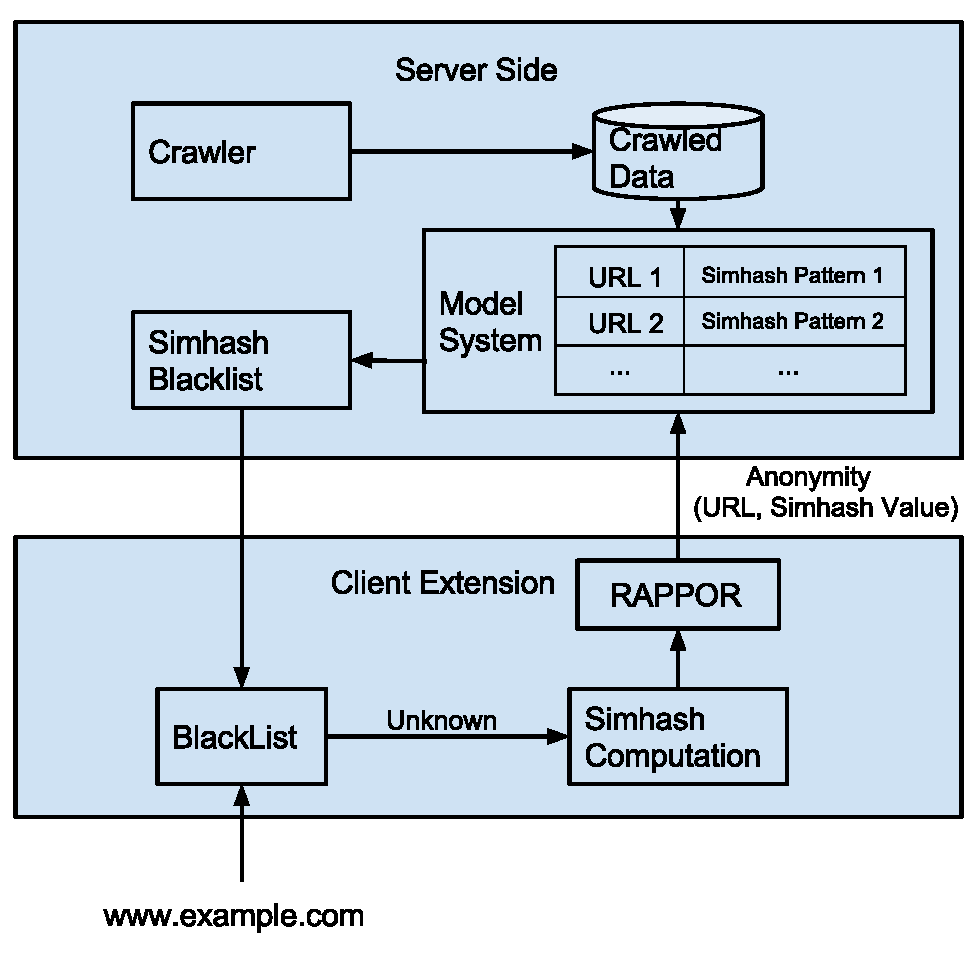
\includegraphics[width=.45\textwidth]{fig/crowdsourcing-cloaking-detection-system}
  \caption{Workflow of crowdsource cloaking detection sysetem}
  \label{fig:workflow}
\end{figure}


The workflow ~\autoref{fig:workflow} is to collect page contents simhash on the user side, and compare
them to simhash of the same link from ad serving company to find cloaking. When
the differences of the simhashes are significantly large, the page is marked
cloaking. We generate two simhash for page content and structure respectively.
Intuition behind this is, simhash difference between different sites are larger
than different visits of the same site. We build a two-phase system to detect
cloaking: cluster learning phase, and cloaking detection phase. In the cluster
learning phase, an ad company visit urls and generate simhash from its content
with its owned IP, and learn pattern and distribution of the simhashes, i.e.
simhash-based website model. In the cloaking detection phase, the ad company
collects simhash from its users. Compare them with learned patterns, return
cloaking score or mismatch



\section{Conclusion}
\label{s:conclusion}

Current solution, multiple pass of data, doesn’t work, and hard to
handle various types of cloaking.
Our model works because …




%
%\section{Acknowledgments}
%
%A polite author always includes acknowledgments.  Thank everyone,
%especially those who funded the work. 
%
%\section{Availability}
%
%It's great when this section says that MyWonderfulApp is free software, 
%available via anonymous FTP from
%
%\begin{center}
%{\tt ftp.site.dom/pub/myname/Wonderful}\\
%\end{center}
%
%Also, it's even greater when you can write that information is also 
%available on the Wonderful homepage at 
%
%\begin{center}
%{\tt http://www.site.dom/\~{}myname/SWIG}
%\end{center}
%
%Now we get serious and fill in those references.  Remember you will
%have to run latex twice on the document in order to resolve those
%cite tags you met earlier.  This is where they get resolved.
%We've preserved some real ones in addition to the template-speak.
%After the bibliography you are DONE.

{\footnotesize \bibliographystyle{acm}
%\bibliography{../common/bibliography}}
\bibliography{ruian,weiren}}

%\theendnotes

\end{document}



